\section{Geometrija na ravnini in v prostoru}

\begin{frame}
    \sectionpage
\end{frame}

\begin{frame}
    \tableofcontents[currentsection, hideothersubsections]
\end{frame}

    \subsection{Osnovni geometrijski pojmi}

        \begin{frame}
            \frametitle{Osnovni geometrijski pojmi}
        \end{frame}

    \subsection{Kot}

        \begin{frame}
            \frametitle{Kot}
        \end{frame}

    \subsection{Konstrukcije matematičnih objektov}

        \begin{frame}
            \frametitle{Konstrukcije matematičnih objektov}
        \end{frame}

    \subsection{Preslikave na ravnini}

        \begin{frame}
            \frametitle{Preslikave na ravnini}

            \large\textbf{Pravokotna projekcija}
            ~\\

            \normalsize
            \begin{columns}
                \column{0.62\textwidth}
                    \begin{alertblock}{}
                        Dani sta točka $T$ in premica $p$. Naj bo $q$ tista pravokotnica na premico $p$, ki poteka skozi točko $T$. 
                        Presečišče $T'$ premice $q$ s premico $p$ imenujemo \textbf{pravokotna projekcija} točke $T$ na premico $p$. 
                        Točka $T'$ je točki $T$ najbližja točka premice $p$. \\
                    \end{alertblock}
                    % ~\\
                    \begin{alertblock}{}
                        \textbf{Razdalja} točke $T$ od premice $p$ je: \\ $\quad \quad \quad \quad d(T,p)=d(T,T')=\left\lvert TT'\right\rvert$. \\
                    \end{alertblock} ~\\

                \column{0.35\textwidth}            
                    % \begin{figure}
                    % 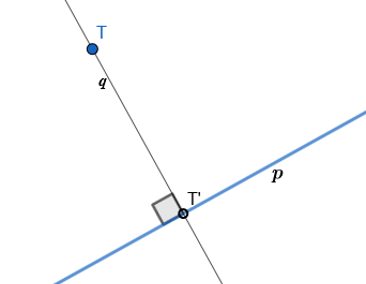
\includegraphics[scale=0.5]{Slike in skice/Pravokotna_projekcija.png}
                    % \end{figure}

                    \begin{figure}
                        \begin{tikzpicture}
                            % \clip (0,0) rectangle (14.000000,10.000000);
                            {\footnotesize
                            
                            % Drawing line Q
                            \draw [line width=0.016cm] (3.000000,1.000000) -- (2.932918,1.134164);%
                            \draw [line width=0.016cm] (2.899377,1.201246) -- (2.832295,1.335410);%
                            \draw [line width=0.016cm] (2.798754,1.402492) -- (2.731672,1.536656);%
                            \draw [line width=0.016cm] (2.698131,1.603738) -- (2.631049,1.737902);%
                            \draw [line width=0.016cm] (2.582111,1.835777) -- (2.530426,1.939149);%
                            \draw [line width=0.016cm] (2.496885,2.006231) -- (2.429803,2.140395);%
                            \draw [line width=0.016cm] (2.396262,2.207477) -- (2.329180,2.341641);%
                            \draw [line width=0.016cm] (2.295639,2.408723) -- (2.228557,2.542887);%
                            \draw [line width=0.016cm] (2.195016,2.609969) -- (2.127933,2.744133);%
                            \draw [line width=0.016cm] (2.094392,2.811215) -- (2.027310,2.945379);%
                            \draw [line width=0.016cm] (1.993769,3.012461) -- (1.926687,3.146625);%
                            \draw [line width=0.016cm] (1.893146,3.213707) -- (1.826064,3.347871);%
                            \draw [line width=0.016cm] (1.792523,3.414953) -- (1.725441,3.549117);%
                            \draw [line width=0.016cm] (1.691900,3.616200) -- (1.624818,3.750364);%
                            \draw [line width=0.016cm] (1.591277,3.817446) -- (1.524195,3.951610);%
                            \draw [line width=0.016cm] (1.482111,4.035777) -- (1.423572,4.152856);%
                            \draw [line width=0.016cm] (1.390031,4.219938) -- (1.322949,4.354102);%
                            \draw [line width=0.016cm] (1.289408,4.421184) -- (1.250000,4.500000);%
                            
                            % Marking point q
                            \draw (1.847000,3.306000) node [anchor=east] { $q$ };%
                            
                            % Marking point T by circle
                            \draw [line width=0.016cm] (1.500000,4.000000) circle (0.040000);%
                            \draw (1.550000,4.000000) node [anchor=south] { $T$ };%
                            
                            % Marking point \frac{\pi}{2}
                            \draw (2.250000,2.000000) node  { $\frac{\pi}{2}$ };%
                            
                            % Changing color 0 0 255
                            \definecolor{r0g0b255}{rgb}{0.000000,0.000000,1.000000}%
                            \color{r0g0b255}% 
                            
                            % Drawing line P
                            \draw [line width=0.016cm] (1.000000,1.000000) -- (2.564223,1.782111);%
                            \draw [line width=0.016cm] (2.635777,1.817889) -- (4.500000,2.750000);%
                            
                            % Marking point p
                            \draw (4.155000,2.578000) node [anchor=north] { $p$ };%
                            
                            % Changing color 255 0 0
                            \definecolor{r255g0b0}{rgb}{1.000000,0.000000,0.000000}%
                            \color{r255g0b0}% 
                            
                            % Marking point T' by circle
                            \draw [line width=0.016cm] (2.600000,1.800000) circle (0.040000);%
                            \draw (2.500000,1.900000) node [anchor=south west] { $T'$ };%
                            \color{black}
                            }
                        \end{tikzpicture}
                    \end{figure}
            \end{columns}

            Pravokotna projekcija daljice $AB$ na premico je daljica $A'B'$, katere krajišči sta pravokotni projekciji točk $A$ in $B$.


            \note{
                TABLA: konstrukcija pravokotne projekcije točke  z ravnilom in šestilom
                \\
                TABLA: konstruckija pravokotne projekcije daljice z ravnilom in šestilom
            }


        \end{frame}

        \begin{frame}
            \large\textbf{Toge preslikave}
            ~\\
            \normalsize

            \begin{alertblock}{}
                \textbf{Toga preslikava} (izometrija) je preslikava v ravnini, ki ohranja razdalje.
                \begin{align*}
                    \tau:~ &A \mapsto A' \\ 
                    \tau:~ &B \mapsto B' \\ 
                    d(A,B)&=d(A',B')
                \end{align*}
            \end{alertblock}

            Med toge preslikave spadajo:
                \begin{itemize}
                    \item \textbf{vzporedni premiki};
                    \item \textbf{zrcaljenje preko premice};
                    \item \textbf{zrcaljenje preko točke};
                    \item \textbf{rotacija okoli točke}.
                \end{itemize}

            Če kombiniramo več togih preslikav, je dobljena preslikava spet toga preslikava.


            \note{
                Tudi poimenovanje skladnostna preslikava.
                
            }

        \end{frame}

        \begin{frame}
            \large\textbf{Vzporedni premik/translacija}
            ~\\

            \normalsize
            \textbf{Vzporedni premik} ali \textbf{translacija} za dano usmerjeno daljico $\overrightarrow{MN}$ preslika točko $T$ v tako točko $T'$, da sta daljici $TT'$ in $MN$ enako dolgi, vzporedni in enako usmerjeni. \\  %(vektorja $\overrightarrow{TT'}$ in $\overrightarrow{AB}$ sta enaka). \\
            
            % \begin{figure}
            %     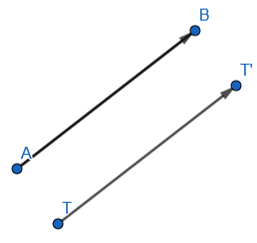
\includegraphics[scale=0.5]{Slike in skice/Vzporedni_premik_tocke.png}
            %     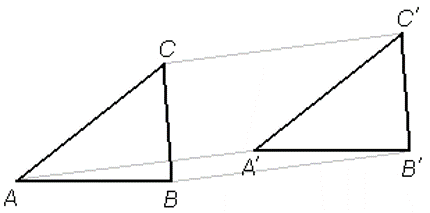
\includegraphics[scale=0.5]{Slike in skice/Vzporedni_premik_trikotnika.png}
            % \end{figure}

            \begin{figure}
                \begin{tikzpicture}
                    % \clip (0,0) rectangle (14.000000,10.000000);
                    {\footnotesize
                    
                    % Drawing segment M N
                    \draw [line width=0.016cm] (1.537947,2.512649) -- (4.462053,3.487351);%
                    
                    % Drawing arrow M N 1.00
                    \draw [line width=0.016cm] (4.205447,3.443092) -- (4.460726,3.492412);%
                    \draw [line width=0.016cm] (4.205447,3.443092) -- (4.405943,3.468648);%
                    \draw [line width=0.016cm] (4.230213,3.368795) -- (4.464028,3.482506);%
                    \draw [line width=0.016cm] (4.230213,3.368795) -- (4.405943,3.468648);%
                    
                    % Drawing segment T T'
                    \draw [line width=0.016cm] (2.037947,1.512649) -- (2.142302,1.547434);%
                    \draw [line width=0.016cm] (2.213454,1.571151) -- (2.355756,1.618585);%
                    \draw [line width=0.016cm] (2.426907,1.642302) -- (2.569210,1.689737);%
                    \draw [line width=0.016cm] (2.640361,1.713454) -- (2.782664,1.760888);%
                    \draw [line width=0.016cm] (2.853815,1.784605) -- (2.996117,1.832039);%
                    \draw [line width=0.016cm] (3.067269,1.855756) -- (3.209571,1.903190);%
                    \draw [line width=0.016cm] (3.280722,1.926907) -- (3.423025,1.974342);%
                    \draw [line width=0.016cm] (3.494176,1.998059) -- (3.636479,2.045493);%
                    \draw [line width=0.016cm] (3.707630,2.069210) -- (3.849932,2.116644);%
                    \draw [line width=0.016cm] (3.921084,2.140361) -- (4.063386,2.187795);%
                    \draw [line width=0.016cm] (4.134537,2.211512) -- (4.276840,2.258947);%
                    \draw [line width=0.016cm] (4.347991,2.282664) -- (4.490294,2.330098);%
                    \draw [line width=0.016cm] (4.561445,2.353815) -- (4.703747,2.401249);%
                    \draw [line width=0.016cm] (4.774899,2.424966) -- (4.917201,2.472400);%
                    
                    % Drawing arrow T T' 1.00
                    \draw [line width=0.016cm] (4.705447,2.443092) -- (4.960726,2.492412);%
                    \draw [line width=0.016cm] (4.705447,2.443092) -- (4.905943,2.468648);%
                    \draw [line width=0.016cm] (4.730213,2.368795) -- (4.964028,2.482506);%
                    \draw [line width=0.016cm] (4.730213,2.368795) -- (4.905943,2.468648);%
                    
                    % Marking point T by circle
                    \draw [line width=0.016cm] (2.000000,1.500000) circle (0.040000);%
                    \draw (2.000000,1.500000) node [anchor=north] { $T$ };%
                    
                    % Marking point A by circle
                    \draw [line width=0.016cm] (6.000000,2.000000) circle (0.040000);%
                    \draw (6.000000,2.000000) node [anchor=north] { $A$ };%
                    
                    % Marking point B by circle
                    \draw [line width=0.016cm] (9.000000,2.000000) circle (0.040000);%
                    \draw (9.000000,2.000000) node [anchor=north] { $B$ };%
                    
                    % Marking point C by circle
                    \draw [line width=0.016cm] (7.000000,4.000000) circle (0.040000);%
                    \draw (7.000000,4.000000) node [anchor=south] { $C$ };%
                    
                    % Drawing segment A B
                    \draw [line width=0.016cm] (6.040000,2.000000) -- (8.960000,2.000000);%
                    
                    % Drawing segment B C
                    \draw [line width=0.016cm] (8.971716,2.028284) -- (7.028284,3.971716);%
                    
                    % Drawing segment A C
                    \draw [line width=0.016cm] (6.017889,2.035777) -- (6.982111,3.964223);%
                    
                    % Drawing segment A' B'
                    \draw [line width=0.016cm] (9.040000,3.000000) -- (11.960000,3.000000);%
                    
                    % Drawing segment B' C'
                    \draw [line width=0.016cm] (11.971716,3.028284) -- (10.028284,4.971716);%
                    
                    % Drawing segment A' C'
                    \draw [line width=0.016cm] (9.017889,3.035777) -- (9.982111,4.964223);%
                    
                    % Drawing segment A A'
                    \draw [line width=0.016cm] (6.037947,2.012649) -- (6.142302,2.047434);%
                    \draw [line width=0.016cm] (6.213454,2.071151) -- (6.355756,2.118585);%
                    \draw [line width=0.016cm] (6.426907,2.142302) -- (6.569210,2.189737);%
                    \draw [line width=0.016cm] (6.640361,2.213454) -- (6.782664,2.260888);%
                    \draw [line width=0.016cm] (6.853815,2.284605) -- (6.996117,2.332039);%
                    \draw [line width=0.016cm] (7.067269,2.355756) -- (7.209571,2.403190);%
                    \draw [line width=0.016cm] (7.280722,2.426907) -- (7.423025,2.474342);%
                    \draw [line width=0.016cm] (7.494176,2.498059) -- (7.636479,2.545493);%
                    \draw [line width=0.016cm] (7.707630,2.569210) -- (7.849932,2.616644);%
                    \draw [line width=0.016cm] (7.921084,2.640361) -- (8.063386,2.687795);%
                    \draw [line width=0.016cm] (8.134537,2.711512) -- (8.276840,2.758947);%
                    \draw [line width=0.016cm] (8.347991,2.782664) -- (8.490294,2.830098);%
                    \draw [line width=0.016cm] (8.561445,2.853815) -- (8.703747,2.901249);%
                    \draw [line width=0.016cm] (8.774899,2.924966) -- (8.917201,2.972400);%
                    
                    % Drawing segment B B'
                    \draw [line width=0.016cm] (9.037947,2.012649) -- (9.142302,2.047434);%
                    \draw [line width=0.016cm] (9.213454,2.071151) -- (9.355756,2.118585);%
                    \draw [line width=0.016cm] (9.426907,2.142302) -- (9.569210,2.189737);%
                    \draw [line width=0.016cm] (9.640361,2.213454) -- (9.782664,2.260888);%
                    \draw [line width=0.016cm] (9.853815,2.284605) -- (9.996117,2.332039);%
                    \draw [line width=0.016cm] (10.067269,2.355756) -- (10.209571,2.403190);%
                    \draw [line width=0.016cm] (10.280722,2.426907) -- (10.423025,2.474342);%
                    \draw [line width=0.016cm] (10.494176,2.498059) -- (10.636479,2.545493);%
                    \draw [line width=0.016cm] (10.707630,2.569210) -- (10.849932,2.616644);%
                    \draw [line width=0.016cm] (10.921084,2.640361) -- (11.063386,2.687795);%
                    \draw [line width=0.016cm] (11.134537,2.711512) -- (11.276840,2.758947);%
                    \draw [line width=0.016cm] (11.347991,2.782664) -- (11.490294,2.830098);%
                    \draw [line width=0.016cm] (11.561445,2.853815) -- (11.703747,2.901249);%
                    \draw [line width=0.016cm] (11.774899,2.924966) -- (11.917201,2.972400);%
                    
                    % Drawing segment C C'
                    \draw [line width=0.016cm] (7.037947,4.012649) -- (7.142302,4.047434);%
                    \draw [line width=0.016cm] (7.213454,4.071151) -- (7.355756,4.118585);%
                    \draw [line width=0.016cm] (7.426907,4.142302) -- (7.569210,4.189737);%
                    \draw [line width=0.016cm] (7.640361,4.213454) -- (7.782664,4.260888);%
                    \draw [line width=0.016cm] (7.853815,4.284605) -- (7.996117,4.332039);%
                    \draw [line width=0.016cm] (8.067269,4.355756) -- (8.209571,4.403190);%
                    \draw [line width=0.016cm] (8.280722,4.426907) -- (8.423025,4.474342);%
                    \draw [line width=0.016cm] (8.494176,4.498059) -- (8.636479,4.545493);%
                    \draw [line width=0.016cm] (8.707630,4.569210) -- (8.849932,4.616644);%
                    \draw [line width=0.016cm] (8.921084,4.640361) -- (9.063386,4.687795);%
                    \draw [line width=0.016cm] (9.134537,4.711512) -- (9.276840,4.758947);%
                    \draw [line width=0.016cm] (9.347991,4.782664) -- (9.490294,4.830098);%
                    \draw [line width=0.016cm] (9.561445,4.853815) -- (9.703747,4.901249);%
                    \draw [line width=0.016cm] (9.774899,4.924966) -- (9.917201,4.972400);%
                    
                    % Changing color 0 0 255
                    \definecolor{r0g0b255}{rgb}{0.000000,0.000000,1.000000}%
                    \color{r0g0b255}% 
                    
                    % Marking point M by circle
                    \draw [line width=0.016cm] (1.500000,2.500000) circle (0.040000);%
                    \draw (1.500000,2.500000) node [anchor=north] { $M$ };%
                    
                    % Marking point N by circle
                    \draw [line width=0.016cm] (4.500000,3.500000) circle (0.040000);%
                    \draw (4.500000,3.500000) node [anchor=south] { $N$ };%
                    
                    % Changing color 255 0 0
                    \definecolor{r255g0b0}{rgb}{1.000000,0.000000,0.000000}%
                    \color{r255g0b0}% 
                    
                    % Marking point T' by circle
                    \draw [line width=0.016cm] (5.000000,2.500000) circle (0.040000);%
                    \draw (5.000000,2.500000) node [anchor=south] { $T'$ };%
                    
                    % Marking point C' by circle
                    \draw [line width=0.016cm] (10.000000,5.000000) circle (0.040000);%
                    \draw (10.000000,5.000000) node [anchor=south] { $C'$ };%
                    
                    % Marking point A' by circle
                    \draw [line width=0.016cm] (9.000000,3.000000) circle (0.040000);%
                    \draw (9.000000,3.000000) node [anchor=north] { $A'$ };%
                    
                    % Marking point B' by circle
                    \draw [line width=0.016cm] (12.000000,3.000000) circle (0.040000);%
                    \draw (12.000000,3.000000) node [anchor=north] { $B'$ };%
                    \color{black}
                    }
                \end{tikzpicture}
                    
            \end{figure}

            Vzporedni premik ohranja orientacijo likov, daljice preslika v enako dolge vzporedne daljice, ohranja velikost kotov, like preslika v skladne like, nima negibnih točk za $\overrightarrow{MN}\neq \overrightarrow{0}$.


            \note{
                TABLA: konstrukcija translacije točke in trikotnika
                \\
                S pomočjo skic na tabli/okviru ugotovitev lastnosti translacije.
            }

        \end{frame}



        % \begin{frame}
            
        %     Če smo kot  odmerili v smeri, ki je nasprotna smeri vrtenja urinega kazalca, smo točko $T$ zavrteli v \textbf{pozitivni smeri} za kot $\alpha$, sicer pa v \textbf{negativni smeri}. 
        %     Namesto smeri vrtenja lahko usmerimo kot: vrtenju v pozitivni smeri ustreza \textbf{pozitivni kot}, vrtenju v negativni smeri pa \textbf{negativni kot}. \\
        %     ~\\


        % \end{frame}


        \begin{frame}
            \large\textbf{Zrcaljenje preko premice}
            ~\\
            ~\\
            \normalsize
            \textbf{Zrcaljenje čez premico} $p$ preslika točko $T$ v tako točko $T'$, da premica $p$ pod pravim kotom razpolavlja daljico $TT'$.
            
            % \begin{figure}
            %     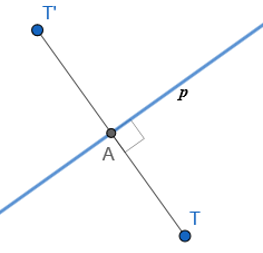
\includegraphics[scale=0.5]{Slike in skice/Zrcaljenje_tocke_cez_premico.png}
            %     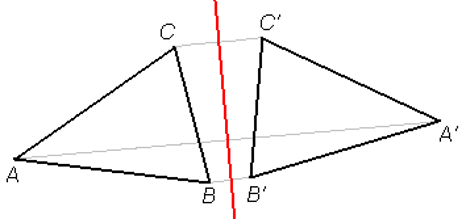
\includegraphics[scale=0.5]{Slike in skice/Zrcaljenje_lika_cez_premico.png}
            % \end{figure}

            \begin{figure}
                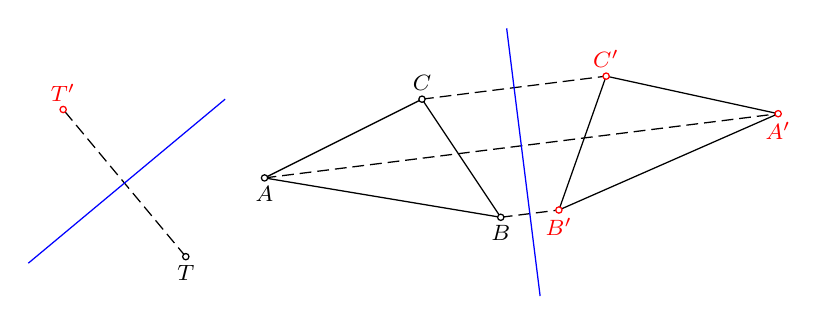
\begin{tikzpicture}
                    % \clip (0,0) rectangle (14.000000,10.000000);
                    {\footnotesize
                    
                    % Marking point T by circle
                    \draw [line width=0.016cm] (3.500000,1.500000) circle (0.040000);%
                    \draw (3.500000,1.500000) node [anchor=north] { $T$ };%
                    
                    % Drawing segment T T'
                    \draw [line width=0.016cm] (3.474393,1.530729) -- (3.403972,1.615233);%
                    \draw [line width=0.016cm] (3.355959,1.672850) -- (3.259931,1.788083);%
                    \draw [line width=0.016cm] (3.211917,1.845700) -- (3.115889,1.960933);%
                    \draw [line width=0.016cm] (3.067876,2.018549) -- (2.971848,2.133783);%
                    \draw [line width=0.016cm] (2.923834,2.191399) -- (2.827806,2.306632);%
                    \draw [line width=0.016cm] (2.779793,2.364249) -- (2.683765,2.479482);%
                    \draw [line width=0.016cm] (2.635751,2.537099) -- (2.539723,2.652332);%
                    \draw [line width=0.016cm] (2.491710,2.709949) -- (2.395682,2.825182);%
                    \draw [line width=0.016cm] (2.347668,2.882798) -- (2.251640,2.998031);%
                    \draw [line width=0.016cm] (2.203627,3.055648) -- (2.107599,3.170881);%
                    \draw [line width=0.016cm] (2.059585,3.228498) -- (1.968230,3.338124);%
                    
                    % Drawing segment C C'
                    \draw [line width=0.016cm] (6.539691,3.504961) -- (6.648842,3.518605);%
                    \draw [line width=0.016cm] (6.723263,3.527908) -- (6.872104,3.546513);%
                    \draw [line width=0.016cm] (6.946525,3.555816) -- (7.095367,3.574421);%
                    \draw [line width=0.016cm] (7.169788,3.583723) -- (7.318629,3.602329);%
                    \draw [line width=0.016cm] (7.393050,3.611631) -- (7.541892,3.630236);%
                    \draw [line width=0.016cm] (7.616313,3.639539) -- (7.765154,3.658144);%
                    \draw [line width=0.016cm] (7.839575,3.667447) -- (7.988417,3.686052);%
                    \draw [line width=0.016cm] (8.062838,3.695355) -- (8.211679,3.713960);%
                    \draw [line width=0.016cm] (8.286100,3.723263) -- (8.434942,3.741868);%
                    \draw [line width=0.016cm] (8.509363,3.751170) -- (8.658204,3.769776);%
                    \draw [line width=0.016cm] (8.732625,3.779078) -- (8.798770,3.787346);%
                    
                    % Drawing segment B B'
                    \draw [line width=0.016cm] (7.539691,2.004961) -- (7.648842,2.018605);%
                    \draw [line width=0.016cm] (7.723263,2.027908) -- (7.872104,2.046513);%
                    \draw [line width=0.016cm] (7.946525,2.055816) -- (8.095367,2.074421);%
                    \draw [line width=0.016cm] (8.169788,2.083723) -- (8.198770,2.087346);%
                    
                    % Drawing segment A A'
                    \draw [line width=0.016cm] (4.539691,2.504961) -- (4.648842,2.518605);%
                    \draw [line width=0.016cm] (4.723263,2.527908) -- (4.872104,2.546513);%
                    \draw [line width=0.016cm] (4.946525,2.555816) -- (5.095367,2.574421);%
                    \draw [line width=0.016cm] (5.169788,2.583723) -- (5.318629,2.602329);%
                    \draw [line width=0.016cm] (5.393050,2.611631) -- (5.541892,2.630236);%
                    \draw [line width=0.016cm] (5.616313,2.639539) -- (5.765154,2.658144);%
                    \draw [line width=0.016cm] (5.839575,2.667447) -- (5.988417,2.686052);%
                    \draw [line width=0.016cm] (6.062838,2.695355) -- (6.211679,2.713960);%
                    \draw [line width=0.016cm] (6.286100,2.723263) -- (6.434942,2.741868);%
                    \draw [line width=0.016cm] (6.509363,2.751170) -- (6.658204,2.769776);%
                    \draw [line width=0.016cm] (6.732625,2.779078) -- (6.881467,2.797683);%
                    \draw [line width=0.016cm] (6.955888,2.806986) -- (7.104729,2.825591);%
                    \draw [line width=0.016cm] (7.179150,2.834894) -- (7.327992,2.853499);%
                    \draw [line width=0.016cm] (7.402413,2.862802) -- (7.551254,2.881407);%
                    \draw [line width=0.016cm] (7.625675,2.890709) -- (7.774517,2.909315);%
                    \draw [line width=0.016cm] (7.848938,2.918617) -- (7.997780,2.937222);%
                    \draw [line width=0.016cm] (8.072200,2.946525) -- (8.221042,2.965130);%
                    \draw [line width=0.016cm] (8.295463,2.974433) -- (8.444305,2.993038);%
                    \draw [line width=0.016cm] (8.518725,3.002341) -- (8.667567,3.020946);%
                    \draw [line width=0.016cm] (8.741988,3.030248) -- (8.890830,3.048854);%
                    \draw [line width=0.016cm] (8.965250,3.058156) -- (9.114092,3.076762);%
                    \draw [line width=0.016cm] (9.188513,3.086064) -- (9.337355,3.104669);%
                    \draw [line width=0.016cm] (9.411775,3.113972) -- (9.560617,3.132577);%
                    \draw [line width=0.016cm] (9.635038,3.141880) -- (9.783880,3.160485);%
                    \draw [line width=0.016cm] (9.858301,3.169788) -- (10.007142,3.188393);%
                    \draw [line width=0.016cm] (10.081563,3.197695) -- (10.230405,3.216301);%
                    \draw [line width=0.016cm] (10.304826,3.225603) -- (10.453667,3.244208);%
                    \draw [line width=0.016cm] (10.528088,3.253511) -- (10.676930,3.272116);%
                    \draw [line width=0.016cm] (10.751351,3.281419) -- (10.900192,3.300024);%
                    \draw [line width=0.016cm] (10.974613,3.309327) -- (10.983386,3.310423);%
                    
                    % Marking point C by circle
                    \draw [line width=0.016cm] (6.500000,3.500000) circle (0.040000);%
                    \draw (6.500000,3.500000) node [anchor=south] { $C$ };%
                    
                    % Marking point A by circle
                    \draw [line width=0.016cm] (4.500000,2.500000) circle (0.040000);%
                    \draw (4.500000,2.500000) node [anchor=north] { $A$ };%
                    
                    % Marking point B by circle
                    \draw [line width=0.016cm] (7.500000,2.000000) circle (0.040000);%
                    \draw (7.500000,2.000000) node [anchor=north] { $B$ };%
                    
                    % Drawing segment A B
                    \draw [line width=0.016cm] (4.539456,2.493424) -- (7.460544,2.006576);%
                    
                    % Drawing segment B C
                    \draw [line width=0.016cm] (7.477812,2.033282) -- (6.522188,3.466718);%
                    
                    % Drawing segment C A
                    \draw [line width=0.016cm] (6.464223,3.482111) -- (4.535777,2.517889);%
                    
                    % Drawing segment C' A'
                    \draw [line width=0.016cm] (8.877541,3.783776) -- (10.983997,3.323916);%
                    
                    % Drawing segment B' C'
                    \draw [line width=0.016cm] (8.251774,2.130027) -- (8.825149,3.754588);%
                    
                    % Drawing segment A' B'
                    \draw [line width=0.016cm] (10.986454,3.299299) -- (8.275085,2.108394);%
                    
                    % Changing color 0 0 255
                    \definecolor{r0g0b255}{rgb}{0.000000,0.000000,1.000000}%
                    \color{r0g0b255}% 
                    
                    % Drawing segment X Y
                    \draw [line width=0.016cm] (4.000000,3.500000) -- (1.500000,1.416667);%
                    
                    % Drawing line r
                    \draw [line width=0.016cm] (8.000000,1.000000) -- (7.575000,4.400000);%
                    
                    % Changing color 255 0 0
                    \definecolor{r255g0b0}{rgb}{1.000000,0.000000,0.000000}%
                    \color{r255g0b0}% 
                    
                    % Marking point T' by circle
                    \draw [line width=0.016cm] (1.942623,3.368852) circle (0.040000);%
                    \draw (1.942623,3.368852) node [anchor=south] { $T'$ };%
                    
                    % Marking point C' by circle
                    \draw [line width=0.016cm] (8.838462,3.792308) circle (0.040000);%
                    \draw (8.838462,3.792308) node [anchor=south] { $C'$ };%
                    
                    % Marking point B' by circle
                    \draw [line width=0.016cm] (8.238462,2.092308) circle (0.040000);%
                    \draw (8.238462,2.092308) node [anchor=north] { $B'$ };%
                    
                    % Marking point A' by circle
                    \draw [line width=0.016cm] (11.023077,3.315385) circle (0.040000);%
                    \draw (11.023077,3.315385) node [anchor=north] { $A'$ };%
                    \color{black}
                    }
                \end{tikzpicture}
                    
            \end{figure}

            Zrcaljenje čez premico daljice preslika v enako dolge daljice, ohranja velikost kotov, ne ohranja orientacije likov, like preslika v skladne like, premic ne preslika v vzporedne premice.

            \note{
                TABLA: konstrukcija zracljenja točke, daljice in trikotnika preko premice
                \\
                S pomočjo skic na tabli/okviru ugotavljanje lastnosti zrcaljenja preko premice.
                \\
                TABLA: Primer enakokrakega trikotnika (osnovnica AC) s simetralo kota z vrhom v C, ki seka c v N. (Dokaz skladnosti trikotnikov ANC in BNC.)
            }
        \end{frame}

        
        \begin{frame}
            \large\textbf{Zrcaljenje preko točke}
            ~\\
            ~\\
            \normalsize
            \textbf{Zrcaljenje čez točko} $O$ preslika točko $T$ v tako točko $T'$, da je $O$ razpolovišče daljice $TT'$. Ta preslikava je enaka vrtenju okrog točke za $180^\circ$.

            % \begin{figure}
            %     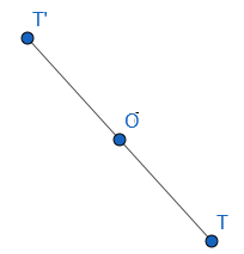
\includegraphics[scale=0.5]{Slike in skice/Zrcaljenje_tocke_cez_tocko.png}
            %     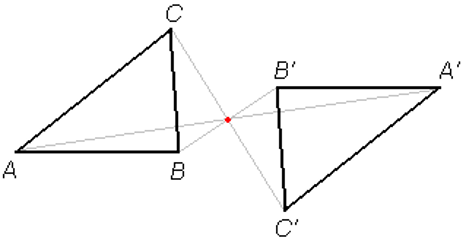
\includegraphics[scale=0.5]{Slike in skice/Zrcaljenje_lika_cez_tocko.png}
            % \end{figure}

            \begin{figure}
                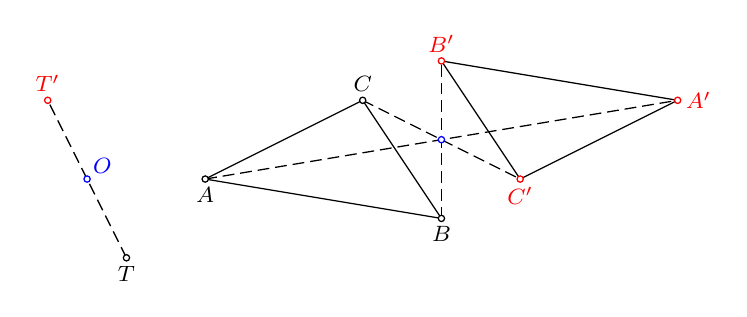
\begin{tikzpicture}
                    % \clip (0,0) rectangle (14.000000,10.000000);
                    {\footnotesize
                    
                    % Marking point T by circle
                    \draw [line width=0.016cm] (3.500000,1.500000) circle (0.040000);%
                    \draw (3.500000,1.500000) node [anchor=north] { $T$ };%
                    
                    % Drawing segment T T'
                    \draw [line width=0.016cm] (3.482111,1.535777) -- (3.432918,1.634164);%
                    \draw [line width=0.016cm] (3.399377,1.701246) -- (3.332295,1.835410);%
                    \draw [line width=0.016cm] (3.298754,1.902492) -- (3.231672,2.036656);%
                    \draw [line width=0.016cm] (3.198131,2.103738) -- (3.131049,2.237902);%
                    \draw [line width=0.016cm] (3.097508,2.304984) -- (3.030426,2.439149);%
                    \draw [line width=0.016cm] (2.982111,2.535777) -- (2.929803,2.640395);%
                    \draw [line width=0.016cm] (2.896262,2.707477) -- (2.829180,2.841641);%
                    \draw [line width=0.016cm] (2.795639,2.908723) -- (2.728557,3.042887);%
                    \draw [line width=0.016cm] (2.695016,3.109969) -- (2.627933,3.244133);%
                    \draw [line width=0.016cm] (2.594392,3.311215) -- (2.527310,3.445379);%
                    
                    % Drawing segment C C'
                    \draw [line width=0.016cm] (6.535777,3.482111) -- (6.634164,3.432918);%
                    \draw [line width=0.016cm] (6.701246,3.399377) -- (6.835410,3.332295);%
                    \draw [line width=0.016cm] (6.902492,3.298754) -- (7.036656,3.231672);%
                    \draw [line width=0.016cm] (7.103738,3.198131) -- (7.237902,3.131049);%
                    \draw [line width=0.016cm] (7.304984,3.097508) -- (7.439149,3.030426);%
                    \draw [line width=0.016cm] (7.535777,2.982111) -- (7.640395,2.929803);%
                    \draw [line width=0.016cm] (7.707477,2.896262) -- (7.841641,2.829180);%
                    \draw [line width=0.016cm] (7.908723,2.795639) -- (8.042887,2.728557);%
                    \draw [line width=0.016cm] (8.109969,2.695016) -- (8.244133,2.627933);%
                    \draw [line width=0.016cm] (8.311215,2.594392) -- (8.445379,2.527310);%
                    
                    % Drawing segment B B'
                    \draw [line width=0.016cm] (7.500000,2.040000) -- (7.500000,2.150000);%
                    \draw [line width=0.016cm] (7.500000,2.225000) -- (7.500000,2.375000);%
                    \draw [line width=0.016cm] (7.500000,2.450000) -- (7.500000,2.600000);%
                    \draw [line width=0.016cm] (7.500000,2.675000) -- (7.500000,2.825000);%
                    \draw [line width=0.016cm] (7.500000,2.900000) -- (7.500000,2.960000);%
                    \draw [line width=0.016cm] (7.500000,3.040000) -- (7.500000,3.050000);%
                    \draw [line width=0.016cm] (7.500000,3.125000) -- (7.500000,3.275000);%
                    \draw [line width=0.016cm] (7.500000,3.350000) -- (7.500000,3.500000);%
                    \draw [line width=0.016cm] (7.500000,3.575000) -- (7.500000,3.725000);%
                    \draw [line width=0.016cm] (7.500000,3.800000) -- (7.500000,3.950000);%
                    
                    % Drawing segment A A'
                    \draw [line width=0.016cm] (4.539456,2.506576) -- (4.647959,2.524660);%
                    \draw [line width=0.016cm] (4.721939,2.536990) -- (4.869898,2.561650);%
                    \draw [line width=0.016cm] (4.943877,2.573980) -- (5.091836,2.598639);%
                    \draw [line width=0.016cm] (5.165816,2.610969) -- (5.313775,2.635629);%
                    \draw [line width=0.016cm] (5.387755,2.647959) -- (5.535714,2.672619);%
                    \draw [line width=0.016cm] (5.609693,2.684949) -- (5.757652,2.709609);%
                    \draw [line width=0.016cm] (5.831632,2.721939) -- (5.979591,2.746598);%
                    \draw [line width=0.016cm] (6.053570,2.758928) -- (6.201530,2.783588);%
                    \draw [line width=0.016cm] (6.275509,2.795918) -- (6.423468,2.820578);%
                    \draw [line width=0.016cm] (6.497448,2.832908) -- (6.645407,2.857568);%
                    \draw [line width=0.016cm] (6.719386,2.869898) -- (6.867345,2.894558);%
                    \draw [line width=0.016cm] (6.941325,2.906887) -- (7.089284,2.931547);%
                    \draw [line width=0.016cm] (7.163264,2.943877) -- (7.311223,2.968537);%
                    \draw [line width=0.016cm] (7.385202,2.980867) -- (7.460544,2.993424);%
                    \draw [line width=0.016cm] (7.607141,3.017857) -- (7.755100,3.042517);%
                    \draw [line width=0.016cm] (7.829079,3.054847) -- (7.977039,3.079506);%
                    \draw [line width=0.016cm] (8.051018,3.091836) -- (8.198977,3.116496);%
                    \draw [line width=0.016cm] (8.272957,3.128826) -- (8.420916,3.153486);%
                    \draw [line width=0.016cm] (8.494895,3.165816) -- (8.642854,3.190476);%
                    \draw [line width=0.016cm] (8.716834,3.202806) -- (8.864793,3.227466);%
                    \draw [line width=0.016cm] (8.938773,3.239795) -- (9.086732,3.264455);%
                    \draw [line width=0.016cm] (9.160711,3.276785) -- (9.308670,3.301445);%
                    \draw [line width=0.016cm] (9.382650,3.313775) -- (9.530609,3.338435);%
                    \draw [line width=0.016cm] (9.604589,3.350765) -- (9.752548,3.375425);%
                    \draw [line width=0.016cm] (9.826527,3.387755) -- (9.974486,3.412414);%
                    \draw [line width=0.016cm] (10.048466,3.424744) -- (10.196425,3.449404);%
                    \draw [line width=0.016cm] (10.270404,3.461734) -- (10.418364,3.486394);%
                    
                    % Marking point C by circle
                    \draw [line width=0.016cm] (6.500000,3.500000) circle (0.040000);%
                    \draw (6.500000,3.500000) node [anchor=south] { $C$ };%
                    
                    % Marking point A by circle
                    \draw [line width=0.016cm] (4.500000,2.500000) circle (0.040000);%
                    \draw (4.500000,2.500000) node [anchor=north] { $A$ };%
                    
                    % Marking point B by circle
                    \draw [line width=0.016cm] (7.500000,2.000000) circle (0.040000);%
                    \draw (7.500000,2.000000) node [anchor=north] { $B$ };%
                    
                    % Drawing segment A B
                    \draw [line width=0.016cm] (4.539456,2.493424) -- (7.460544,2.006576);%
                    
                    % Drawing segment B C
                    \draw [line width=0.016cm] (7.477812,2.033282) -- (6.522188,3.466718);%
                    
                    % Drawing segment C A
                    \draw [line width=0.016cm] (6.464223,3.482111) -- (4.535777,2.517889);%
                    
                    % Drawing segment C' A'
                    \draw [line width=0.016cm] (8.535777,2.517889) -- (10.464223,3.482111);%
                    
                    % Drawing segment B' C'
                    \draw [line width=0.016cm] (7.522188,3.966718) -- (8.477812,2.533282);%
                    
                    % Drawing segment A' B'
                    \draw [line width=0.016cm] (10.460544,3.506576) -- (7.539456,3.993424);%
                    
                    % Changing color 0 0 255
                    \definecolor{r0g0b255}{rgb}{0.000000,0.000000,1.000000}%
                    \color{r0g0b255}% 
                    
                    % Marking point O by circle
                    \draw [line width=0.016cm] (3.000000,2.500000) circle (0.040000);%
                    \draw (2.970000,2.470000) node [anchor=south west] { $O$ };%
                    
                    % Marking point r by circle
                    \draw [line width=0.016cm] (7.500000,3.000000) circle (0.040000);%
                    
                    % Changing color 255 0 0
                    \definecolor{r255g0b0}{rgb}{1.000000,0.000000,0.000000}%
                    \color{r255g0b0}% 
                    
                    % Marking point T' by circle
                    \draw [line width=0.016cm] (2.500000,3.500000) circle (0.040000);%
                    \draw (2.500000,3.500000) node [anchor=south] { $T'$ };%
                    
                    % Marking point C' by circle
                    \draw [line width=0.016cm] (8.500000,2.500000) circle (0.040000);%
                    \draw (8.500000,2.500000) node [anchor=north] { $C'$ };%
                    
                    % Marking point B' by circle
                    \draw [line width=0.016cm] (7.500000,4.000000) circle (0.040000);%
                    \draw (7.500000,4.000000) node [anchor=south] { $B'$ };%
                    
                    % Marking point A' by circle
                    \draw [line width=0.016cm] (10.500000,3.500000) circle (0.040000);%
                    \draw (10.500000,3.500000) node [anchor=west] { $A'$ };%
                    \color{black}
                    }
                \end{tikzpicture}
                    
            \end{figure}

            Zrcaljenje čez točko daljice preslika v enako dolge daljice, ohranja velikosti kotov in orientacijo likov, like preslika v skladne like, premice preslika v vzporedne premice.

            \note{
                TABLA: konstrukcija zracljenja točke in trikotnika preko točke
                \\
                S pomočjo skic na tabli/okviru ugotavljanje lastnosti zrcaljenja preko točke.
            }
        \end{frame}



        \begin{frame}
            \large\textbf{Simetrija}
            ~\\
            \normalsize
            \begin{columns}
                \column{0.65\textwidth}
                ~\\
                Množica točk $\mathcal{M}$ je \textbf{simetrična/somerna glede na premico} $p$, če se pri zrcaljenju čez premico $p$ preslika sama vase. Premico $p$ imenujemo \textbf{simetrala}, \textbf{somernica}, \textbf{simetrijska os} množice $\mathcal{M}$. \\
                 ~\\      
                 ~\\      
                Množica točk $\mathcal{M}$ je \textbf{središčno simetrična/somerna glede na točko} $T$, če se pri zrcaljenju čez točko $T$ preslika sama vase. Točko $T$ imenujemo \textbf{center simetrije} množice $\mathcal{M}$. 
                \column{0.32\textwidth}
                \begin{figure}
                    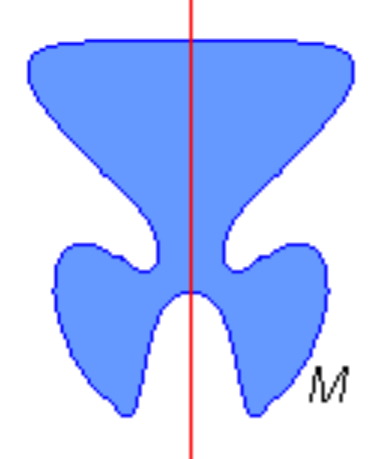
\includegraphics[scale=0.25]{Slike in skice/Simetrija glede na premico.png}

                    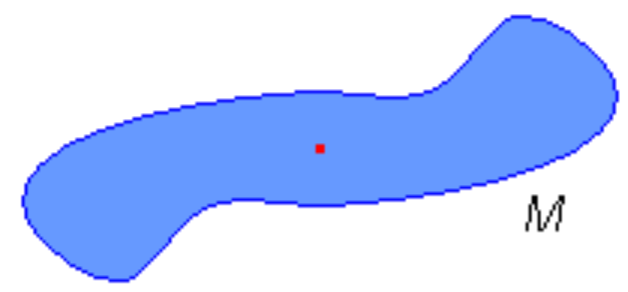
\includegraphics[scale=0.25]{Slike in skice/Simetrija glede na točko.png}
                \end{figure}
            \end{columns}


            \note{
                Ponovitev definicije in konstrukcije simetrale daljice in simetrale kota.
            }
        \end{frame}

        \begin{frame}
            \large\textbf{Rotacija/vrtenje okoli točke}
            ~\\
            \normalsize
            \onslide<2->{
                \textbf{Vrtenje} ali \textbf{zasuk} oziroma \textbf{rotacija} za kot $\varphi$ okrog točke $O$ preslika točko $T$ v točko $T'$, da velja: $\left\lvert OT\right\rvert = \left\lvert OT'\right\rvert$  in $\angle TOT' = \varphi$.
            }

            % \begin{figure}
            %     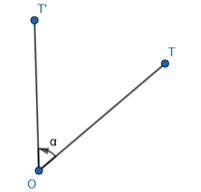
\includegraphics[scale=0.6]{Slike in skice/Rotacija tocke_okoli_tocke.png}
            %     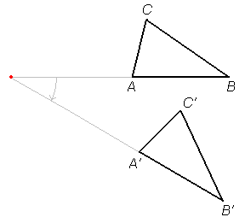
\includegraphics[scale=0.6]{Slike in skice/Rotacija_lika_okoli_tocke.png}
            % \end{figure}

            \pause
            \begin{figure}
                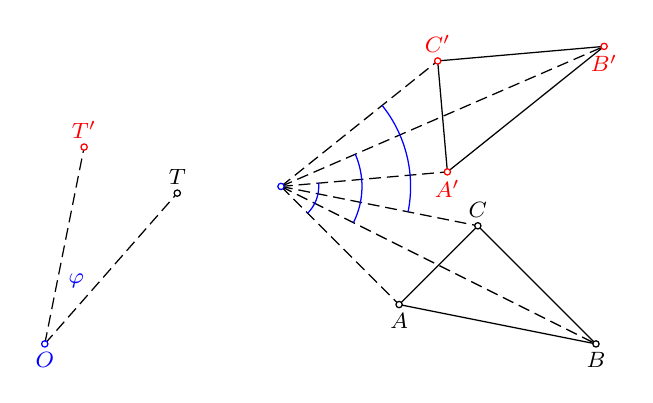
\begin{tikzpicture}
                    % \clip (0,0) rectangle (14.000000,10.000000);
                    {\footnotesize
                    
                    % Drawing segment O T
                    \draw<4-> [line width=0.016cm] (1.526405,1.530046) -- (1.599020,1.612672);%
                    \draw<4-> [line width=0.016cm] (1.648530,1.669009) -- (1.747550,1.781681);%
                    \draw<4-> [line width=0.016cm] (1.797059,1.838017) -- (1.896079,1.950690);%
                    \draw<4-> [line width=0.016cm] (1.945589,2.007026) -- (2.044609,2.119698);%
                    \draw<4-> [line width=0.016cm] (2.094119,2.176035) -- (2.193139,2.288707);%
                    \draw<4-> [line width=0.016cm] (2.242649,2.345043) -- (2.341668,2.457716);%
                    \draw<4-> [line width=0.016cm] (2.391178,2.514052) -- (2.490198,2.626724);%
                    \draw<4-> [line width=0.016cm] (2.539708,2.683060) -- (2.638728,2.795733);%
                    \draw<4-> [line width=0.016cm] (2.688238,2.852069) -- (2.787258,2.964742);%
                    \draw<4-> [line width=0.016cm] (2.836768,3.021078) -- (2.935787,3.133750);%
                    \draw<4-> [line width=0.016cm] (2.985297,3.190086) -- (3.084317,3.302759);%
                    \draw<4-> [line width=0.016cm] (3.133827,3.359095) -- (3.156608,3.385017);%
                    
                    % Drawing segment O T'
                    \draw<5-> [line width=0.016cm] (1.507845,1.539223) -- (1.529417,1.647087);%
                    \draw<5-> [line width=0.016cm] (1.544126,1.720631) -- (1.573544,1.867718);%
                    \draw<5-> [line width=0.016cm] (1.588252,1.941261) -- (1.617670,2.088348);%
                    \draw<5-> [line width=0.016cm] (1.632378,2.161892) -- (1.661796,2.308979);%
                    \draw<5-> [line width=0.016cm] (1.676505,2.382523) -- (1.705922,2.529610);%
                    \draw<5-> [line width=0.016cm] (1.720631,2.603153) -- (1.750048,2.750240);%
                    \draw<5-> [line width=0.016cm] (1.764757,2.823784) -- (1.794174,2.970871);%
                    \draw<5-> [line width=0.016cm] (1.808883,3.044415) -- (1.838300,3.191502);%
                    \draw<5-> [line width=0.016cm] (1.853009,3.265045) -- (1.882426,3.412132);%
                    \draw<5-> [line width=0.016cm] (1.897135,3.485676) -- (1.926553,3.632763);%
                    \draw<5-> [line width=0.016cm] (1.941261,3.706307) -- (1.970679,3.853394);%
                    \draw<5-> [line width=0.016cm] (1.985387,3.926937) -- (1.992155,3.960777);%
                    
                    % Marking point C by circle
                    \draw<6-> [line width=0.016cm] (7.000000,3.000000) circle (0.040000);%
                    \draw<6-> (7.000000,3.000000) node [anchor=south] { $C$ };%
                    
                    % Marking point A by circle
                    \draw<6-> [line width=0.016cm] (6.000000,2.000000) circle (0.040000);%
                    \draw<6-> (6.000000,2.000000) node [anchor=north] { $A$ };%
                    
                    % Marking point B by circle
                    \draw<6-> [line width=0.016cm] (8.500000,1.500000) circle (0.040000);%
                    \draw<6-> (8.500000,1.500000) node [anchor=north] { $B$ };%
                    
                    % Drawing segment A B
                    \draw<6-> [line width=0.016cm] (6.039223,1.992155) -- (8.460777,1.507845);%
                    
                    % Drawing segment B C
                    \draw<6-> [line width=0.016cm] (8.471716,1.528284) -- (7.028284,2.971716);%
                    
                    % Drawing segment A C
                    \draw<6-> [line width=0.016cm] (6.028284,2.028284) -- (6.971716,2.971716);%
                    
                    % Drawing segment X A
                    \draw<7-> [line width=0.016cm] (4.528284,3.471716) -- (4.606066,3.393934);%
                    \draw<7-> [line width=0.016cm] (4.659099,3.340901) -- (4.765165,3.234835);%
                    \draw<7-> [line width=0.016cm] (4.818198,3.181802) -- (4.924264,3.075736);%
                    \draw<7-> [line width=0.016cm] (4.977297,3.022703) -- (5.083363,2.916637);%
                    \draw<7-> [line width=0.016cm] (5.136396,2.863604) -- (5.242462,2.757538);%
                    \draw<7-> [line width=0.016cm] (5.295495,2.704505) -- (5.401561,2.598439);%
                    \draw<7-> [line width=0.016cm] (5.454594,2.545406) -- (5.560660,2.439340);%
                    \draw<7-> [line width=0.016cm] (5.613693,2.386307) -- (5.719759,2.280241);%
                    \draw<7-> [line width=0.016cm] (5.772792,2.227208) -- (5.878858,2.121142);%
                    \draw<7-> [line width=0.016cm] (5.931891,2.068109) -- (5.971716,2.028284);%
                    
                    % Drawing segment X B
                    \draw<7-> [line width=0.016cm] (4.535777,3.482111) -- (4.634164,3.432918);%
                    \draw<7-> [line width=0.016cm] (4.701246,3.399377) -- (4.835410,3.332295);%
                    \draw<7-> [line width=0.016cm] (4.902492,3.298754) -- (5.036656,3.231672);%
                    \draw<7-> [line width=0.016cm] (5.103738,3.198131) -- (5.237902,3.131049);%
                    \draw<7-> [line width=0.016cm] (5.304984,3.097508) -- (5.439149,3.030426);%
                    \draw<7-> [line width=0.016cm] (5.506231,2.996885) -- (5.640395,2.929803);%
                    \draw<7-> [line width=0.016cm] (5.707477,2.896262) -- (5.841641,2.829180);%
                    \draw<7-> [line width=0.016cm] (5.908723,2.795639) -- (6.042887,2.728557);%
                    \draw<7-> [line width=0.016cm] (6.109969,2.695016) -- (6.244133,2.627933);%
                    \draw<7-> [line width=0.016cm] (6.311215,2.594392) -- (6.445379,2.527310);%
                    \draw<7-> [line width=0.016cm] (6.512461,2.493769) -- (6.646625,2.426687);%
                    \draw<7-> [line width=0.016cm] (6.713707,2.393146) -- (6.847871,2.326064);%
                    \draw<7-> [line width=0.016cm] (6.914953,2.292523) -- (7.049117,2.225441);%
                    \draw<7-> [line width=0.016cm] (7.116200,2.191900) -- (7.250364,2.124818);%
                    \draw<7-> [line width=0.016cm] (7.317446,2.091277) -- (7.451610,2.024195);%
                    \draw<7-> [line width=0.016cm] (7.518692,1.990654) -- (7.652856,1.923572);%
                    \draw<7-> [line width=0.016cm] (7.719938,1.890031) -- (7.854102,1.822949);%
                    \draw<7-> [line width=0.016cm] (7.921184,1.789408) -- (8.055348,1.722326);%
                    \draw<7-> [line width=0.016cm] (8.122430,1.688785) -- (8.256594,1.621703);%
                    \draw<7-> [line width=0.016cm] (8.323676,1.588162) -- (8.457840,1.521080);%
                    
                    % Drawing segment X C
                    \draw<7-> [line width=0.016cm] (4.539223,3.492155) -- (4.647087,3.470583);%
                    \draw<7-> [line width=0.016cm] (4.720631,3.455874) -- (4.867718,3.426456);%
                    \draw<7-> [line width=0.016cm] (4.941261,3.411748) -- (5.088348,3.382330);%
                    \draw<7-> [line width=0.016cm] (5.161892,3.367622) -- (5.308979,3.338204);%
                    \draw<7-> [line width=0.016cm] (5.382523,3.323495) -- (5.529610,3.294078);%
                    \draw<7-> [line width=0.016cm] (5.603153,3.279369) -- (5.750240,3.249952);%
                    \draw<7-> [line width=0.016cm] (5.823784,3.235243) -- (5.970871,3.205826);%
                    \draw<7-> [line width=0.016cm] (6.044415,3.191117) -- (6.191502,3.161700);%
                    \draw<7-> [line width=0.016cm] (6.265045,3.146991) -- (6.412132,3.117574);%
                    \draw<7-> [line width=0.016cm] (6.485676,3.102865) -- (6.632763,3.073447);%
                    \draw<7-> [line width=0.016cm] (6.706307,3.058739) -- (6.853394,3.029321);%
                    \draw<7-> [line width=0.016cm] (6.926937,3.014613) -- (6.960777,3.007845);%
                    
                    % Drawing segment A' B'
                    \draw<10-> [line width=0.016cm] (6.644470,3.709889) -- (8.572018,5.253598);%
                    
                    % Drawing segment B' C'
                    \draw<10-> [line width=0.016cm] (8.563392,5.275116) -- (6.529839,5.097203);%
                    
                    % Drawing segment A' C'
                    \draw<10-> [line width=0.016cm] (6.609762,3.724733) -- (6.493478,5.053869);%
                    
                    % Drawing segment X A'
                    \draw<8-> [line width=0.016cm] (4.539848,3.503486) -- (4.649429,3.513073);%
                    \draw<8-> [line width=0.016cm] (4.724144,3.519610) -- (4.873573,3.532683);%
                    \draw<8-> [line width=0.016cm] (4.948288,3.539220) -- (5.097717,3.552293);%
                    \draw<8-> [line width=0.016cm] (5.172431,3.558830) -- (5.321861,3.571903);%
                    \draw<8-> [line width=0.016cm] (5.396575,3.578440) -- (5.546004,3.591513);%
                    \draw<8-> [line width=0.016cm] (5.620719,3.598050) -- (5.770148,3.611124);%
                    \draw<8-> [line width=0.016cm] (5.844863,3.617660) -- (5.994292,3.630734);%
                    \draw<8-> [line width=0.016cm] (6.069007,3.637270) -- (6.218436,3.650344);%
                    \draw<8-> [line width=0.016cm] (6.293150,3.656880) -- (6.442580,3.669954);%
                    \draw<8-> [line width=0.016cm] (6.517294,3.676490) -- (6.573400,3.681399);%
                    
                    % Drawing segment X B'
                    \draw<8-> [line width=0.016cm] (4.536700,3.515908) -- (4.637627,3.559656);%
                    \draw<8-> [line width=0.016cm] (4.706440,3.589484) -- (4.844067,3.649140);%
                    \draw<8-> [line width=0.016cm] (4.912881,3.678968) -- (5.050507,3.738625);%
                    \draw<8-> [line width=0.016cm] (5.119321,3.768453) -- (5.256948,3.828109);%
                    \draw<8-> [line width=0.016cm] (5.325761,3.857937) -- (5.463388,3.917593);%
                    \draw<8-> [line width=0.016cm] (5.532201,3.947421) -- (5.669828,4.007077);%
                    \draw<8-> [line width=0.016cm] (5.738642,4.036905) -- (5.876268,4.096561);%
                    \draw<8-> [line width=0.016cm] (5.945082,4.126389) -- (6.082709,4.186046);%
                    \draw<8-> [line width=0.016cm] (6.151522,4.215874) -- (6.289149,4.275530);%
                    \draw<8-> [line width=0.016cm] (6.357962,4.305358) -- (6.495589,4.365014);%
                    \draw<8-> [line width=0.016cm] (6.564403,4.394842) -- (6.702029,4.454498);%
                    \draw<8-> [line width=0.016cm] (6.770843,4.484326) -- (6.908470,4.543982);%
                    \draw<8-> [line width=0.016cm] (6.977283,4.573810) -- (7.114910,4.633467);%
                    \draw<8-> [line width=0.016cm] (7.183723,4.663295) -- (7.321350,4.722951);%
                    \draw<8-> [line width=0.016cm] (7.390164,4.752779) -- (7.527790,4.812435);%
                    \draw<8-> [line width=0.016cm] (7.596604,4.842263) -- (7.734231,4.901919);%
                    \draw<8-> [line width=0.016cm] (7.803044,4.931747) -- (7.940671,4.991403);%
                    \draw<8-> [line width=0.016cm] (8.009484,5.021232) -- (8.147111,5.080888);%
                    \draw<8-> [line width=0.016cm] (8.215925,5.110716) -- (8.353551,5.170372);%
                    \draw<8-> [line width=0.016cm] (8.422365,5.200200) -- (8.559992,5.259856);%
                    
                    % Drawing segment X C'
                    \draw<8-> [line width=0.016cm] (4.531222,3.525004) -- (4.617081,3.593766);%
                    \draw<8-> [line width=0.016cm] (4.675621,3.640649) -- (4.792702,3.734415);%
                    \draw<8-> [line width=0.016cm] (4.851242,3.781298) -- (4.968323,3.875064);%
                    \draw<8-> [line width=0.016cm] (5.026864,3.921947) -- (5.143945,4.015714);%
                    \draw<8-> [line width=0.016cm] (5.202485,4.062597) -- (5.319566,4.156363);%
                    \draw<8-> [line width=0.016cm] (5.378106,4.203246) -- (5.495187,4.297012);%
                    \draw<8-> [line width=0.016cm] (5.553727,4.343895) -- (5.670808,4.437661);%
                    \draw<8-> [line width=0.016cm] (5.729349,4.484544) -- (5.846429,4.578310);%
                    \draw<8-> [line width=0.016cm] (5.904970,4.625193) -- (6.022051,4.718959);%
                    \draw<8-> [line width=0.016cm] (6.080591,4.765842) -- (6.197672,4.859608);%
                    \draw<8-> [line width=0.016cm] (6.256212,4.906491) -- (6.373293,5.000258);%
                    \draw<8-> [line width=0.016cm] (6.431834,5.047141) -- (6.458770,5.068713);%
                    
                    % Marking point T by circle
                    \draw<3-> [line width=0.016cm] (3.183013,3.415063) circle (0.040000);%
                    \draw<3-> (3.183013,3.415063) node [anchor=south] { $T$ };%
                    
                    % Changing color 0 0 255
                    \definecolor{r0g0b255}{rgb}{0.000000,0.000000,1.000000}%
                    \color{r0g0b255}% 
                    
                    % Marking point O by circle
                    \draw<3-> [line width=0.016cm] (1.500000,1.500000) circle (0.040000);%
                    \draw<3-> (1.500000,1.500000) node [anchor=north] { $O$ };%
                    
                    % Marking point \alpha
                    \draw<5-> (1.900000,2.300000) node  { $\varphi$ };%
                    
                    % Marking point X by circle
                    \draw<6-> [line width=0.016cm] (4.500000,3.500000) circle (0.040000);%
                    
                    % Drawing arc X a 50.00
                    \draw<8-> [line width=0.016cm] (4.839000,3.161000) -- (4.839000,3.161000) arc (315:360:0.479418 and 0.479418) --(4.979418,3.500000) arc (0:4:0.479418 and 0.479418) -- (4.977594,3.541784);%
                    
                    % Drawing arc X b 50.00
                    \draw<8-> [line width=0.016cm] (5.420000,3.040000) -- (5.424492,3.049095) arc (334:360:1.028591 and 1.028591) --(5.528591,3.500000) arc (0:23:1.028591 and 1.028591) -- (5.443745,3.909079);%
                    
                    % Drawing arc X c 50.00
                    \draw<8-> [line width=0.016cm] (6.114000,3.177000) -- (6.115761,3.185927) arc (349:360:1.646003 and 1.646003) --(6.146003,3.500000) arc (0:38:1.646003 and 1.646003) -- (5.784892,4.528775);%
                    
                    % Changing color 255 0 0
                    \definecolor{r255g0b0}{rgb}{1.000000,0.000000,0.000000}%
                    \color{r255g0b0}% 
                    
                    % Marking point T' by circle
                    \draw<5-> [line width=0.016cm] (2.000000,4.000000) circle (0.040000);%
                    \draw<5-> (2.000000,4.000000) node [anchor=south] { $T'$ };%
                    
                    % Marking point A' by circle
                    \draw<9-> [line width=0.016cm] (6.613248,3.684885) circle (0.040000);%
                    \draw<9-> (6.613248,3.684885) node [anchor=north] { $A'$ };%
                    
                    % Marking point B' by circle
                    \draw<9-> [line width=0.016cm] (8.603239,5.278602) circle (0.040000);%
                    \draw<9-> (8.603239,5.278602) node [anchor=north] { $B'$ };%
                    
                    % Marking point C' by circle
                    \draw<9-> [line width=0.016cm] (6.489991,5.093717) circle (0.040000);%
                    \draw<9-> (6.489991,5.093717) node [anchor=south] { $C'$ };%
                    \color{black}
                    }
                \end{tikzpicture}
            \end{figure}

            \onslide<11->{Vrtenje okoli točke preslika daljice v enako dolge daljice, ohranja velikosti kotov in orientacijo likov, like preslika v skladne like, premic pa ne preslika v vzporedne premice.} 


            \note{
                TABLA: konstrukcija rotacije točke okoli točke za nek kot; rotacija trikotnika za isti kot
                \\
                Opomba: vrtenje v pozitivni/negativni smeri oziroma za pozitiven/negativen kot
                \\
                S pomočjo skic na tabli/okviru ugotovitev lastnosti dane prelikave.

            }
        \end{frame}


        \begin{frame}

            \begin{exampleblock}{Naloga}
                Konstruiraj daljico $AB$ poljubne dolžine. Konstruiraj še:
                \begin{itemize}
                    \item točko $C$, ki jo dobiš tako, da točko $B$ zavrtiš okrog točke $A$ za kot $120^\circ$;
                    \item točko $D$, ki je pravokotna projekcija točke $C$ na nosilko daljice $AB$;
                    \item zrcalno sliko točke $C$ glede na točko $B$ in dobljeno točko označi $C'$;
                    \item simetralo kota z vrhom v $B$, katerega kraka potekata skozi $C$ in $C'$.
                \end{itemize}
            \end{exampleblock}

        \end{frame}
        \note{
            Priredba nalog 57 in 58 v Matematika 2 (Zbirka nalog ...).
        }
    \subsection{Trikotnik}

        \begin{frame}
            \frametitle{Trikotnik}

            \pause
            \begin{alertblock}{}
                \textbf{Trikotnik} je lik/množica točk v ravnini, omejena s tremi daljicami -- \textbf{stranice} ($a, b, c$), ki povezujejo tri nekolinearne točke ($A, B, C$) v ravnini. Te točke imenujemo \textbf{oglišča} trikotnika.
            \end{alertblock}
            
            % \begin{figure}
            %     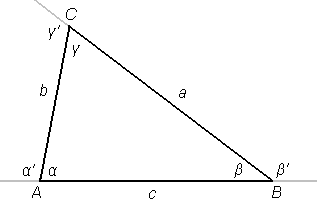
\includegraphics[scale=0.7]{Slike in skice/Trikotnik.png}    
            % \end{figure}

            \begin{figure}
                
                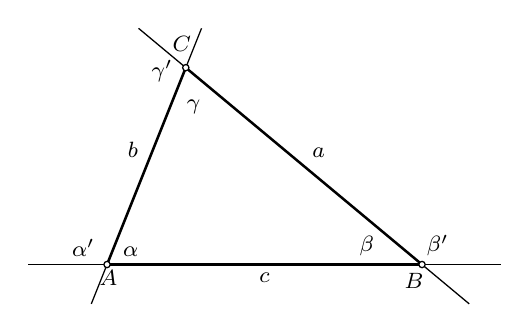
\begin{tikzpicture}
                    % \clip (0,0) rectangle (14.000000,10.000000);
                    {\footnotesize
                    
                    % Marking point A by circle
                    \draw<2-> [line width=0.016cm] (2.000000,1.500000) circle (0.040000);%
                    \draw<2-> (1.800000,1.530000) node [anchor=north west] { $A$ };%
                    
                    % Marking point B by circle
                    \draw<2-> [line width=0.016cm] (6.000000,1.500000) circle (0.040000);%
                    \draw<2-> (5.900000,1.500000) node [anchor=north] { $B$ };%
                    
                    % Marking point C by circle
                    \draw<2-> [line width=0.016cm] (3.000000,4.000000) circle (0.040000);%
                    \draw<2-> (2.950000,4.100000) node [anchor=south] { $C$ };%
                    
                    % Drawing line A B
                    \draw<4-> [line width=0.016cm] (1.000000,1.500000) -- (1.960000,1.500000);%
                    \draw<4-> [line width=0.016cm] (2.040000,1.500000) -- (5.960000,1.500000);%
                    \draw<4-> [line width=0.016cm] (6.040000,1.500000) -- (7.000000,1.500000);%
                    
                    % Drawing line B C
                    \draw<4-> [line width=0.016cm] (6.600000,1.000000) -- (6.030729,1.474393);%
                    \draw<4-> [line width=0.016cm] (5.969271,1.525607) -- (3.030729,3.974393);%
                    \draw<4-> [line width=0.016cm] (2.969271,4.025607) -- (2.400000,4.500000);%
                    
                    % Drawing line A C
                    \draw<4-> [line width=0.016cm] (1.800000,1.000000) -- (1.985144,1.462861);%
                    \draw<4-> [line width=0.016cm] (2.014856,1.537139) -- (2.985144,3.962861);%
                    \draw<4-> [line width=0.016cm] (3.014856,4.037139) -- (3.200000,4.500000);%
                    
                    % Marking point c
                    \draw<2-> (4.000000,1.500000) node [anchor=north] { $c$ };%
                    
                    % Marking point a
                    \draw<2-> (4.500000,2.750000) node [anchor=south west] { $a$ };%
                    
                    % Marking point b
                    \draw<2-> (2.500000,2.750000) node [anchor=south east] { $b$ };%
                    
                    % Marking point \gamma
                    \draw<3-> (3.100000,3.700000) node [anchor=north] { $\gamma$ };%
                    
                    % Marking point \gamma'
                    \draw<4-> (2.700000,4.200000) node [anchor=north] { $\gamma'$ };%
                    
                    % Marking point \beta
                    \draw<3-> (5.300000,1.500000) node [anchor=south] { $\beta$ };%
                    
                    % Marking point \beta'
                    \draw<4-> (6.200000,1.500000) node [anchor=south] { $\beta'$ };%
                    
                    % Marking point \alpha
                    \draw<3-> (2.300000,1.500000) node [anchor=south] { $\alpha$ };%
                    
                    % Marking point \alpha'
                    \draw<4-> (1.700000,1.500000) node [anchor=south] { $\alpha'$ };%
                    
                    % Drawing segment A B
                    \draw<2-> [line width=0.032cm] (2.040000,1.500000) -- (5.960000,1.500000);%
                    
                    % Drawing segment B C
                    \draw<2-> [line width=0.032cm] (5.969271,1.525607) -- (3.030729,3.974393);%
                    
                    % Drawing segment A C
                    \draw<2-> [line width=0.032cm] (2.014856,1.537139) -- (2.985144,3.962861);%
                    }
                \end{tikzpicture}
            \end{figure}

            \onslide<3->{V trikotniku $\triangle ABC$  so $\alpha, \beta$ in $\gamma$ \textbf{notranji koti},} \onslide<4->{njihovi sokoti $\alpha', \beta'$ in $\gamma'$ pa so \textbf{zunanji koti}. }
            

        \end{frame}


        \begin{frame}
            
            \begin{alertblock}{}
                Vsota notranjih kotov trikotnika je $180^\circ$: $$\alpha+\beta+\gamma=180^\circ.$$ 
            \end{alertblock}

            \pause
            \begin{alertblock}{}
                Zunanji kot trikotnika je enak vsoti notranjih nepriležnih kotov: 
                \begin{align*}
                    \alpha' &= \beta+\gamma \\
                    \beta' &= \alpha+\gamma \\
                    \gamma' &= \alpha+\beta
                \end{align*}
            \end{alertblock}

            \pause
            \begin{alertblock}{}
                Vsota zunanjih kotov trikotnika je $360^\circ$: $$\alpha'+\beta'+\gamma'=360^\circ.$$ 
            \end{alertblock}


            \note{
                DOKAZ 1. izreka: Upoštevamo lastnosti kotov z vzporednimi kraki. Narišemo nosilko stranice $a$ preko oglišča $C$. Konstruiramo vzpordnico k $c$ skozi $C$. Dobljena kota sta skladna $\alpha$ oziroma $\beta$. Vsi trije koti skupaj tvorijo iztegnjeni kot ($180^\circ$).
                \\
                DOKAZ 2. izreka: Dokaz naredimo zgolj za enega izmed kotov: Na skici dokaz prejšnjega izreka vidimo, da je zunanji kot pri oglišču $C$ enak vsoti kotov $\alpha$ in $\beta$.
                \\
                DOKAZ 3. izreka: Po prejšnjih dveh izrekih sledi, da je $\alpha'+\beta'+\gamma'=2\cdot(\alpha+\beta+\gamma)=2\cdot180^\circ=360^\circ$.
            }
        \end{frame}


        \begin{frame}
            \begin{exampleblock}{Naloga 65}
                Izračunaj velikosti notranjih in zunanjih kotov trikotnika $\triangle ABC$, če je $\alpha= 67^\circ 13'$ in $\beta' = 133^\circ 25'$.
            \end{exampleblock}

            \pause
            \begin{exampleblock}{Naloga 68}
                Velikosti notranjih kotov trikotnika so v razmerju $2:5:11$. V kolikšnem razmerju so velikosti zunanjih kotov tega trikotnika?
            \end{exampleblock}

            \pause
            \begin{exampleblock}{Naloga 70}
                Notranji kot ob oglišču $A$ trikotnika $\triangle ABC$ je za $1^\circ$ manjši od velikosti notranjega kota ob oglišču $C$.  Zunanji kot v oglišču $C$ je za $1^\circ$ večji od dvakratnika velikosti notranjega kota ob oglišču $A$. Izračunaj velikosti notranjih kotov trikotnika $\triangle ABC$.
            \end{exampleblock}
        \end{frame}
        

        \begin{frame}
            
            \begin{alertblock}{}
                Nasproti daljše stranice trikotnika leži večji notranji kot, nasproti krajše stranice pa manjši notranji kot trikotnika.
                $$a>b \Leftrightarrow \alpha > \beta$$
            \end{alertblock}

            \pause
            \begin{alertblock}{Trikotniška neenakost}
                Vsaka stranica trikotnika je krajša od vsote dolžin drugih dveh stranic.
                \begin{align*}
                    a &< b + c \\
                    b &< a + c \\
                    c &< a + b
                \end{align*}
            \end{alertblock}

            % \begin{alertblock}{}
            %     Vsaka stranica trikotnika je daljša od absolutne vrednosti razlike dolžin drugih dveh stranic.
            % \end{alertblock}


            \note{
                DOKAZ 1. izreka: Denimo, da je $c$ daljša od $b$ v trikotniku $ABC$. Konstruiramo simetralo $\alpha$ in označimo presečišče z $a$ z $D$. Daljico $AC$ prenesemo na $AB$ in točko označimo z $E$. Dobili smo skladna trikotnika $AED$ in $ACD$ (skupna $AD$, $|AC|=|AE|$, kot med njima). Torej je $\angle DEA = \gamma$ zunanji kot za trikotnik $EBD$, torej enak vsoti $\beta$ in $\angle EDB$. To pomeni da velja $\gamma > \beta$.
                \\
                DOKAZ 2. izreka: Dokaz naredimo zgolj za eno neenakost: Podaljšamo eno izmed stranic trikotnika $ABC$, naj bo to $a$, preko oglišča $C$ za dolžino stranice $b$. Dobili smo enakokrak trikotnik $ACC'$, skladna kota $\angle CAC'$ in $\angle AC'C$ označimo z $\varphi$. Kot $\angle BAC' = \epsilon$ je večji od $\varphi$. V trikotniku $ABC'$ je $\epsilon > \varphi$, zato je $BC' > c$. To nam da: $c<a+b$.
            }
        \end{frame}


        \begin{frame}
            \begin{exampleblock}{Naloga 76}
                Ali obstaja trikotnik z danimi dolžinami stranic?
                \begin{enumerate}
                    \item $a=4~cm,\ b=5~cm,\ c=10~cm$;
                    \item $a=4~cm,\ b=5~cm,\ c=8~cm$;
                    \item $a=5~cm,\ b=12~cm,\ c=6~cm$.
                \end{enumerate}
            \end{exampleblock}

            \pause
            \begin{exampleblock}{Naloga 77}
                Po velikosti uredi notranje kote trikotnika $\triangle ABC$.
                \begin{enumerate}
                    \item $a=33~dm,\ b=22~dm,\ c=28~dm$;
                    \item $a=32~m,\ b=35~m,\ c=38~m$;
                \end{enumerate}
            \end{exampleblock}

        \end{frame}


        \begin{frame}

            \begin{alertblock}{}
                \textbf{Višina} na stranico trikotnika je daljica, ki povezuje nosilko te stranice z nasprotnim ogliščem in je pravokotna na to nosilko. 
                Njena dolžina je razdalja oglišča od nasprotne stranice.
            \end{alertblock}

            % \begin{figure}
            %     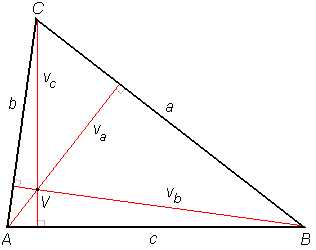
\includegraphics[scale=0.5]{Slike in skice/Visina_in_visinska_tocka.png}
            % \end{figure}
            
            \begin{figure}
                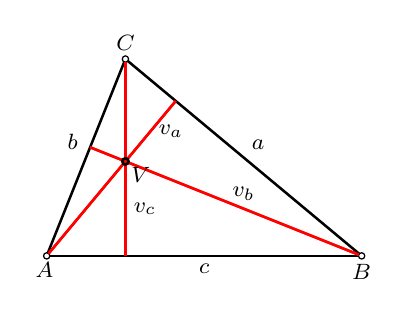
\begin{tikzpicture}
                    % \clip (0,0) rectangle (14.000000,10.000000);
                    {\footnotesize
                    
                    % Marking point A by circle
                    \draw<1-> [line width=0.016cm] (2.000000,1.500000) circle (0.040000);%
                    \draw<1-> (1.970000,1.530000) node [anchor=north] { $A$ };%
                    
                    % Marking point B by circle
                    \draw<1-> [line width=0.016cm] (6.000000,1.500000) circle (0.040000);%
                    \draw<1-> (6.000000,1.500000) node [anchor=north] { $B$ };%
                    
                    % Marking point C by circle
                    \draw<1-> [line width=0.016cm] (3.000000,4.000000) circle (0.040000);%
                    \draw<1-> (3.000000,4.000000) node [anchor=south] { $C$ };%
                    
                    % Marking point c
                    \draw<1-> (4.000000,1.500000) node [anchor=north] { $c$ };%
                    
                    % Marking point a
                    \draw<1-> (4.500000,2.750000) node [anchor=south west] { $a$ };%
                    
                    % Marking point b
                    \draw<1-> (2.500000,2.750000) node [anchor=south east] { $b$ };%
                    
                    % Marking point v_a
                    \draw<2-> (3.319672,3.083607) node [anchor=west] { $v_a$ };%
                    
                    % Marking point v_c
                    \draw<2-> (3.000000,2.100000) node [anchor=west] { $v_c$ };%
                    
                    % Marking point v_b
                    \draw<2-> (4.500000,2.100000) node [anchor=south] { $v_b$ };%
                    
                    % Drawing segment A B
                    \draw<1-> [line width=0.032cm] (2.040000,1.500000) -- (5.960000,1.500000);%
                    
                    % Drawing segment B C
                    \draw<1-> [line width=0.032cm] (5.969271,1.525607) -- (3.030729,3.974393);%
                    
                    % Drawing segment A C
                    \draw<1-> [line width=0.032cm] (2.014856,1.537139) -- (2.985144,3.962861);%
                    
                    % Changing color 255 0 0
                    \definecolor{r255g0b0}{rgb}{1.000000,0.000000,0.000000}%
                    \color{r255g0b0}% 
                    
                    % Drawing segment A A'
                    \draw<2> [line width=0.032cm] (2.025607,1.530729) -- (3.639344,3.467213);%
                    \draw<3-> [line width=0.032cm] (2.025607,1.530729) -- (2.974393,2.669271);%
                    \draw<3-> [line width=0.032cm] (3.025607,2.730729) -- (3.639344,3.467213);%
                    
                    % Drawing segment B B'
                    \draw<2> [line width=0.032cm] (5.962861,1.514856) -- (2.551724,2.879310);%
                    \draw<3-> [line width=0.032cm] (5.962861,1.514856) -- (3.037139,2.685144);%
                    \draw<3-> [line width=0.032cm] (2.962861,2.714856) -- (2.551724,2.879310);%
                    
                    % Drawing segment C C'
                    \draw<2> [line width=0.032cm] (3.000000,3.960000) -- (3.000000,1.500000);%
                    \draw<3-> [line width=0.032cm] (3.000000,3.960000) -- (3.000000,2.740000);%
                    \draw<3-> [line width=0.032cm] (3.000000,2.660000) -- (3.000000,1.500000);%
                    
                    % Changing color 0 0 0
                    \definecolor{r0g0b0}{rgb}{0.000000,0.000000,0.000000}%
                    \color{r0g0b0}% 
                    
                    % Marking point V by circle
                    \draw<3-> [line width=0.032cm] (3.000000,2.700000) circle (0.040000);%
                    \draw<3-> (2.970000,2.730000) node [anchor=north west] { $V$ };%
                    \color{black}
                    }
                \end{tikzpicture}
                    
            \end{figure}

            \onslide<3->{
            \begin{alertblock}{}
                Nosilke vseh treh višin na stranice trikotnika se sekajo v eni točki, ki jo imenujemo \textbf{višinska točka} ali \textbf{ortocenter}.
            \end{alertblock}
            }


            \note{
                TABLA: konstrukcija višin trikotnika z ravnilom in šestilom
                \\
                DOKAZ: Skozi vsako oglišče trikotnika narišemo vzporednico k nasprotni stranici. Presečišča označimo z $A', B', C'$. Zaradi vzporednosti sta štirkotnika $ABA'C$ in $ABCB'$ paralelograma, torej je $|AB|=|A'C|$ in $|AB|=|B'C|$, iz tega $|A'C|=|B'C|$: $C$ razpolavlja $A'B'$. Podobno za $B$ in $A$. Noslike višin trikotnika $ABC$ so simmetrale stranic trikotnika $A'B'C'$. Te se sekajo v središču očrtane krožnice trikotnika $A'B'C'$, ki je višinska točka trikotnika $ABC$.

            }
        \end{frame}


        \begin{frame}

            \begin{alertblock}{}
                \textbf{Težiščnica} na stranico trikotnika je daljica, ki povezuje razpolovišče te stranice z nasprotnim ogliščem. 
            \end{alertblock}

            % \begin{figure}
            %     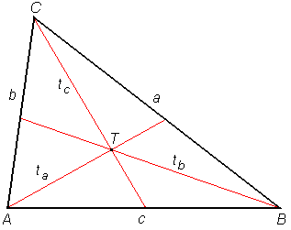
\includegraphics[scale=0.5]{Slike in skice/Teziscnice_in_tezisce.png}
            % \end{figure}

            \begin{figure}
                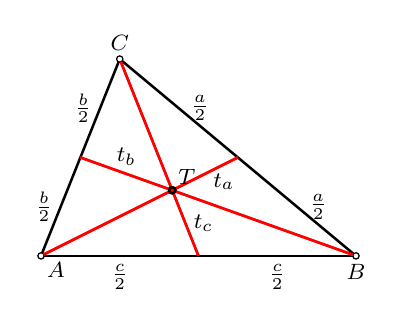
\begin{tikzpicture}
                    % \clip (0,0) rectangle (14.000000,10.000000);
                    {\footnotesize
                    
                    % Marking point A by circle
                    \draw [line width=0.016cm] (2.000000,1.500000) circle (0.040000);%
                    \draw (1.970000,1.530000) node [anchor=north west] { $A$ };%
                    
                    % Marking point B by circle
                    \draw [line width=0.016cm] (6.000000,1.500000) circle (0.040000);%
                    \draw (6.000000,1.500000) node [anchor=north] { $B$ };%
                    
                    % Marking point C by circle
                    \draw [line width=0.016cm] (3.000000,4.000000) circle (0.040000);%
                    \draw (3.000000,4.000000) node [anchor=south] { $C$ };%
                    
                    % Marking point t_a
                    \draw<2-> (4.083333,2.441667) node [anchor=west] { $t_a$ };%
                    
                    % Marking point t_c
                    \draw<2-> (3.833333,1.916667) node [anchor=west] { $t_c$ };%
                    
                    % Marking point t_b
                    \draw<2-> (3.083333,2.541667) node [anchor=south] { $t_b$ };%
                    
                    % Marking point \frac{b}{2}
                    \draw<2-> (2.250000,2.125000) node [anchor=east] { $\frac{b}{2}$ };%
                    
                    % Marking point \frac{b}{2}
                    \draw<2-> (2.750000,3.375000) node [anchor=east] { $\frac{b}{2}$ };%
                    
                    % Marking point \frac{c}{2}
                    \draw<2-> (3.000000,1.500000) node [anchor=north] { $\frac{c}{2}$ };%
                    
                    % Marking point \frac{c}{2}
                    \draw<2-> (5.000000,1.500000) node [anchor=north] { $\frac{c}{2}$ };%
                    
                    % Marking point \frac{a}{2}
                    \draw<2-> (5.30000,2.125000) node [anchor=west] { $\frac{a}{2}$ };%
                    
                    % Marking point \frac{a}{2}
                    \draw<2-> (3.80000,3.375000) node [anchor=west] { $\frac{a}{2}$ };%
                    
                    % Drawing segment A B
                    \draw [line width=0.032cm] (2.040000,1.500000) -- (5.960000,1.500000);%
                    
                    % Drawing segment B C
                    \draw [line width=0.032cm] (5.969271,1.525607) -- (3.030729,3.974393);%
                    
                    % Drawing segment A C
                    \draw [line width=0.032cm] (2.014856,1.537139) -- (2.985144,3.962861);%
                    
                    % Changing color 255 0 0
                    \definecolor{r255g0b0}{rgb}{1.000000,0.000000,0.000000}%
                    \color{r255g0b0}% 
                    
                    % Drawing segment A a
                    \draw<2> [line width=0.032cm] (2.035777,1.517889) -- (4.500000,2.750000);%
                    \draw<3-> [line width=0.032cm] (2.035777,1.517889) -- (3.630890,2.315445);%
                    \draw<3-> [line width=0.032cm] (3.702444,2.351222) -- (4.500000,2.750000);%
                    
                    % Drawing segment B b
                    \draw<2> [line width=0.032cm] (5.962330,1.513453) -- (2.500000,2.750000);%
                    \draw<3-> [line width=0.032cm] (5.962330,1.513453) -- (3.704336,2.319880);%
                    \draw<3-> [line width=0.032cm] (3.628997,2.346787) -- (2.500000,2.750000);%
                    
                    % Drawing segment C c
                    \draw<2> [line width=0.032cm] (3.014856,3.962861) -- (4.000000,1.500000);%
                    \draw<3-> [line width=0.032cm] (3.014856,3.962861) -- (3.651811,2.370472);%
                    \draw<3-> [line width=0.032cm] (3.681522,2.296194) -- (4.000000,1.500000);%
                    
                    % Changing color 0 0 0
                    \definecolor{r0g0b0}{rgb}{0.000000,0.000000,0.000000}%
                    \color{r0g0b0}% 
                    
                    % Marking point T by circle
                    \draw<3-> [line width=0.032cm] (3.666667,2.333333) circle (0.040000);%
                    \draw<3-> (3.636667,2.303333) node [anchor=south west] { $T$ };%
                    \color{black}
                    }
                \end{tikzpicture}
                    
            \end{figure}

            \onslide<3->{
            \begin{alertblock}{}
                Vse tri trikotnikove težiščnice se sekajo v eni točki -- \textbf{težišču} ali \textbf{baricentru} trikotnika. \\ 
                Težišče deli težiščnico v razmerju $1:2$.
            \end{alertblock}
            }

            \note{
                TABLA: konstrukcija težišnic z ravnilom in šestilom
            }

        \end{frame}


        \begin{frame}
            \begin{exampleblock}{Naloga 81}
                Konstruiraj trikotnik.
                \begin{itemize}
                    \item $a=2~cm,\ b=6~cm,\ c=5~cm$;
                    \item $c=4~cm,\ \alpha=60^\circ,\ \beta=45^\circ$;
                    \item $a=4~cm,\ c=5~cm,\ \alpha=45^\circ$;
                    \item $a=2,5~cm,\ c=5~cm,\ v_c=2~cm$;
                    \item $v_c=3~cm,\ \alpha=60^\circ,\ \beta=75^\circ$;
                    \item $v_a=2~cm,\ v_b=4~cm,\ \gamma=45^\circ$;
                    \item $b=65~cm,\ t_b=3,5~cm,\ \gamma=60^\circ$;
                    \item $v_a=3~cm,\ t_c=4~cm,\ \beta=45^\circ$.
                \end{itemize}
            \end{exampleblock}


            \note{
                Morda manj primerov pri nalogi 81. (b, c, h, l, n, r, š, u)
            }
        \end{frame}


        \begin{frame}

            \begin{alertblock}{}
                Simetrale vseh treh stranic trikotnika se sekajo v eni točki. Ta točka je \textbf{središče trikotniku očrtane krožnice}. 
            \end{alertblock}

            % \begin{figure}
            %     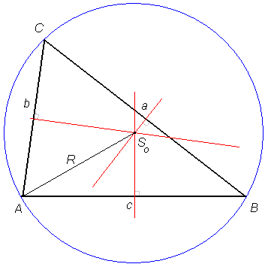
\includegraphics[scale=0.55]{Slike in skice/Trikotniku_ocrtana_kroznica.png}
            % \end{figure}

            \begin{figure}
                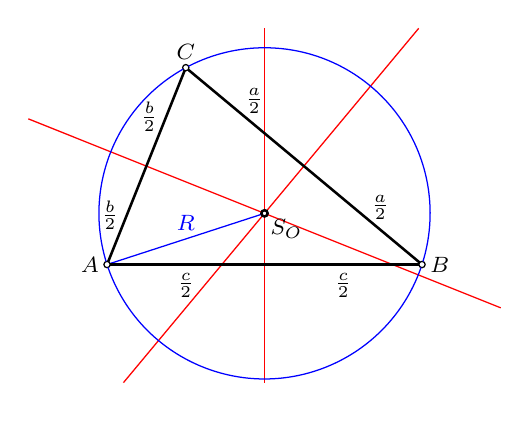
\begin{tikzpicture}
                    % \clip (0,0) rectangle (14.000000,10.000000);
                    {\footnotesize
                    
                    % Marking point A by circle
                    \draw [line width=0.016cm] (2.000000,2.500000) circle (0.040000);%
                    \draw (2.000000,2.500000) node [anchor=east] { $A$ };%
                    
                    % Marking point B by circle
                    \draw [line width=0.016cm] (6.000000,2.500000) circle (0.040000);%
                    \draw (6.000000,2.500000) node [anchor=west] { $B$ };%
                    
                    % Marking point C by circle
                    \draw [line width=0.016cm] (3.000000,5.000000) circle (0.040000);%
                    \draw (3.000000,5.000000) node [anchor=south] { $C$ };%
                    
                    % Marking point \frac{b}{2}
                    \draw (2.250000,3.125000) node [anchor=east] { $\frac{b}{2}$ };%
                    
                    % Marking point \frac{b}{2}
                    \draw (2.750000,4.375000) node [anchor=east] { $\frac{b}{2}$ };%
                    
                    % Marking point \frac{c}{2}
                    \draw (3.000000,2.500000) node [anchor=north] { $\frac{c}{2}$ };%
                    
                    % Marking point \frac{c}{2}
                    \draw (5.000000,2.500000) node [anchor=north] { $\frac{c}{2}$ };%
                    
                    % Marking point \frac{a}{2}
                    \draw (5.250000,3.225000) node [anchor=west] { $\frac{a}{2}$ };%
                    
                    % Marking point \frac{a}{2}
                    \draw (3.650000,4.575000) node [anchor=west] { $\frac{a}{2}$ };%
                    
                    % Changing color 255 0 0
                    \definecolor{r255g0b0}{rgb}{1.000000,0.000000,0.000000}%
                    \color{r255g0b0}% 
                    
                    % Drawing line s_c
                    \draw [line width=0.016cm] (4.000000,1.000000) -- (4.000000,3.110000);%
                    \draw [line width=0.016cm] (4.000000,3.190000) -- (4.000000,5.500000);%
                    
                    % Drawing line s_a
                    \draw [line width=0.016cm] (2.208333,1.000000) -- (3.974393,3.119271);%
                    \draw [line width=0.016cm] (4.025607,3.180729) -- (5.958333,5.500000);%
                    
                    % Drawing line s_b
                    \draw [line width=0.016cm] (1.000000,4.350000) -- (3.962861,3.164856);%
                    \draw [line width=0.016cm] (4.037139,3.135144) -- (7.000000,1.950000);%
                    
                    % Changing color 0 0 255
                    \definecolor{r0g0b255}{rgb}{0.000000,0.000000,1.000000}%
                    \color{r0g0b255}% 
                    
                    % Drawing circle S_O A
                    \draw [line width=0.016cm] (2.012724,2.462079) -- (2.023851,2.430741) arc (200:340:2.102974 and 2.102974) -- (5.987275,2.462077);%
                    \draw [line width=0.016cm] (6.012001,2.538157) -- (6.021508,2.570341) arc (344:360:2.102974 and 2.102974) --(6.102974,3.150000) arc (0:117:2.102974 and 2.102974) -- (3.035368,5.018685);%
                    \draw [line width=0.016cm] (2.964994,4.980646) -- (2.948513,4.971229) arc (120:196:2.102974 and 2.102974) -- (1.987999,2.538158);%
                    
                    % Drawing segment A S_O
                    \draw [line width=0.016cm] (2.038041,2.512363) -- (3.961959,3.137637);%
                    
                    % Marking point R
                    \draw (3.000000,2.825000) node [anchor=south] { $R$ };%
                    
                    % Changing color 0 0 0
                    \definecolor{r0g0b0}{rgb}{0.000000,0.000000,0.000000}%
                    \color{r0g0b0}% 
                    
                    % Drawing segment A B
                    \draw [line width=0.032cm] (2.040000,2.500000) -- (5.960000,2.500000);%
                    
                    % Drawing segment B C
                    \draw [line width=0.032cm] (5.969271,2.525607) -- (3.030729,4.974393);%
                    
                    % Drawing segment A C
                    \draw [line width=0.032cm] (2.014856,2.537139) -- (2.985144,4.962861);%
                    
                    % Marking point S_O by circle
                    \draw [line width=0.032cm] (4.000000,3.150000) circle (0.040000);%
                    \draw (3.970000,3.180000) node [anchor=north west] { $S_O$ };%
                    \color{black}
                    }
                \end{tikzpicture}    

            \end{figure}

            \pause
            Očrtana krožnica poteka skozi vsa tri oglišča trikotnika. Vse tri stranice trikotnika so tetive te krožnice.


            \note{
                TABLA: konstrukcija simetral stranic in očrtane krožnice z ravnilom in šestilom
                \\
                DOKAZ: Konstruiramo simetrali stranic $AC$ in $AB$. Vsaka točka na njiju je enako oddaljena od oglišč stranice. Torej je njuno presečišče $S_O$ enako oddalje od vseh trh oglišč $A, B, C$ in tako središče trikotniku očrtane krožnice. Podbno za simetralo strannice $BC$.
            }
        \end{frame}


        \begin{frame}

            \begin{alertblock}{}
                Simetrale notranjih kotov trikotnika se sekajo v eni točki. Ta točka je \textbf{središče trikotniku včrtane krožnice}.
            \end{alertblock}

            % \begin{figure}
            %     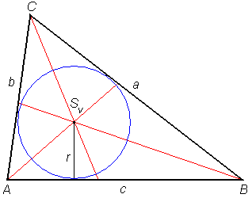
\includegraphics[scale=0.65]{Slike in skice/Trikotniku_vcrtana_kroznica.png}
            % \end{figure}

            \begin{figure}
                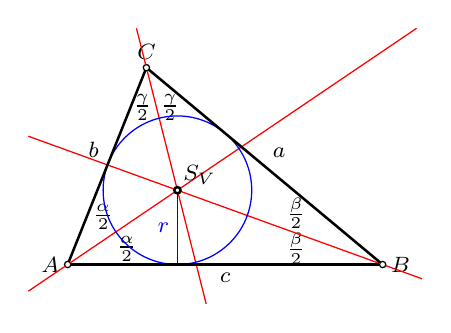
\begin{tikzpicture}
                    % \clip (0,0) rectangle (14.000000,10.000000);
                    {\footnotesize
                    
                    % Marking point A by circle
                    \draw [line width=0.016cm] (2.000000,2.500000) circle (0.040000);%
                    \draw (2.000000,2.500000) node [anchor=east] { $A$ };%
                    
                    % Marking point B by circle
                    \draw [line width=0.016cm] (6.000000,2.500000) circle (0.040000);%
                    \draw (6.000000,2.500000) node [anchor=west] { $B$ };%
                    
                    % Marking point C by circle
                    \draw [line width=0.016cm] (3.000000,5.000000) circle (0.040000);%
                    \draw (3.000000,5.000000) node [anchor=south] { $C$ };%
                    
                    % Marking point b
                    \draw (2.500000,3.750000) node [anchor=south east] { $b$ };%
                    
                    % Marking point c
                    \draw (4.000000,2.500000) node [anchor=north] { $c$ };%
                    
                    % Marking point a
                    \draw (4.500000,3.750000) node [anchor=south west] { $a$ };%
                    
                    % Marking point \frac{\alpha}{2}
                    \draw (2.750000,2.700000) node  { $\frac{\alpha}{2}$ };%
                    
                    % Marking point \frac{\gamma}{2}
                    \draw (2.950000,4.500000) node  { $\frac{\gamma}{2}$ };%
                    
                    % Marking point \frac{\alpha}{2}
                    \draw (2.450000,3.100000) node  { $\frac{\alpha}{2}$ };%
                    
                    % Marking point \frac{\beta}{2}
                    \draw (4.900000,2.700000) node  { $\frac{\beta}{2}$ };%
                    
                    % Marking point \frac{\beta}{2}
                    \draw (4.900000,3.150000) node  { $\frac{\beta}{2}$ };%
                    
                    % Marking point \frac{\gamma}{2}
                    \draw (3.300000,4.500000) node  { $\frac{\gamma}{2}$ };%
                    
                    % Changing color 255 0 0
                    \definecolor{r255g0b0}{rgb}{1.000000,0.000000,0.000000}%
                    \color{r255g0b0}% 
                    
                    % Drawing line s_c
                    \draw [line width=0.016cm] (3.758922,2.000000) -- (3.403539,3.404822);%
                    \draw [line width=0.016cm] (3.383919,3.482379) -- (3.009810,4.961222);%
                    \draw [line width=0.016cm] (2.990190,5.038778) -- (2.873513,5.500000);%
                    
                    % Drawing line s_a
                    \draw [line width=0.016cm] (6.431099,5.500000) -- (3.426851,3.466025);%
                    \draw [line width=0.016cm] (3.360606,3.421175) -- (2.033123,2.522425);%
                    \draw [line width=0.016cm] (1.966877,2.477575) -- (1.500000,2.161484);%
                    
                    % Drawing line s_b
                    \draw [line width=0.016cm] (1.500000,4.129225) -- (3.356118,3.457217);%
                    \draw [line width=0.016cm] (3.431340,3.429983) -- (5.962389,2.513617);%
                    \draw [line width=0.016cm] (6.037611,2.486383) -- (6.500000,2.318975);%
                    
                    % Changing color 0 0 255
                    \definecolor{r0g0b255}{rgb}{0.000000,0.000000,1.000000}%
                    \color{r0g0b255}% 
                    
                    % Drawing circle S_V X
                    \draw [line width=0.016cm] (3.393729,3.443600) circle (0.943600);%
                    
                    % Drawing segment X S_V
                    \draw [line width=0.016cm] (3.393729,2.500000) -- (3.393729,3.403600);%
                    
                    % Marking point r
                    \draw (3.393729,2.971800) node [anchor=east] { $r$ };%
                    
                    % Changing color 0 0 0
                    \definecolor{r0g0b0}{rgb}{0.000000,0.000000,0.000000}%
                    \color{r0g0b0}% 
                    
                    % Drawing segment A B
                    \draw [line width=0.032cm] (2.040000,2.500000) -- (5.960000,2.500000);%
                    
                    % Drawing segment B C
                    \draw [line width=0.032cm] (5.969271,2.525607) -- (3.030729,4.974393);%
                    
                    % Drawing segment A C
                    \draw [line width=0.032cm] (2.014856,2.537139) -- (2.985144,4.962861);%
                    
                    % Marking point S_V by circle
                    \draw [line width=0.032cm] (3.393729,3.443600) circle (0.040000);%
                    \draw (3.363729,3.413600) node [anchor=south west] { $S_V$ };%
                    \color{black}
                    }
                \end{tikzpicture}
                    
            \end{figure}
            
            \pause
            Včrtana krožnica ima vse tri stranice trikotnika za tangente.


            \note{
                TABLA: konstrukcija simetral kotov in včrtane krožnice z ravnilom in šestilom
                \\
                DOKAZ: Narišemo simetrali kotov pri $A$ in $B$. Vsaka točka na njiju je enako oddaljena od nosilk stranic ob kotu. Njuno presečišče $S_V$ je torej enako oddalje od vseh treh nosilk stranic trikotnika. In zatorej je središče krožnice, ki se dotika vseh treh stranic -- trikotniku včrtane krožnice.
            }
        \end{frame}

        \begin{frame}
            \begin{exampleblock}{Naloga 83}
                Dan je trikotnik $\triangle ABC$ s podatki $b=5~cm,\ \beta=45^\circ,\ \gamma=60^\circ$.
                \begin{enumerate}
                    \item Konstruiraj trikotnik $\triangle ABC$.
                    \item Konstruiraj trikotniku $\triangle ABC$ očrtano krožnico.
                    \item Koliko je velik zunanji kot pri oglišču $A$?
                \end{enumerate}
            \end{exampleblock}

            \pause
            \begin{exampleblock}{Naloga 84}
                Dan je trikotnik $\triangle ABC$ s podatki $a=5~cm,\ c=4~cm,\ t_c=4~cm$.
                \begin{enumerate}
                    \item Konstruiraj trikotnik $\triangle ABC$.
                    \item Konstruiraj trikotniku $\triangle ABC$ včrtano krožnico.
                    \item Kateri izmed $\angle BAC$ in $\angle ACB$ je večji? Utemelji (brez merjenja).
                \end{enumerate}
            \end{exampleblock}
        \end{frame}


        \begin{frame}

            \begin{alertblock}{}
                Težišče, središče trikotniku očrtane kroznice, središče trikotniku včrtane krožnice in višinska točka so \textbf{znamenite točke trikotnika}.

            \end{alertblock}

            \pause
            \begin{alertblock}{}
                Višinska točka, središče očrtane krožnice in težišče so vedno kolinearne. Premico, ki jih povezuje, imenujemo \textbf{Eulerjeva premica}.
            \end{alertblock}

            % \begin{figure}
            %     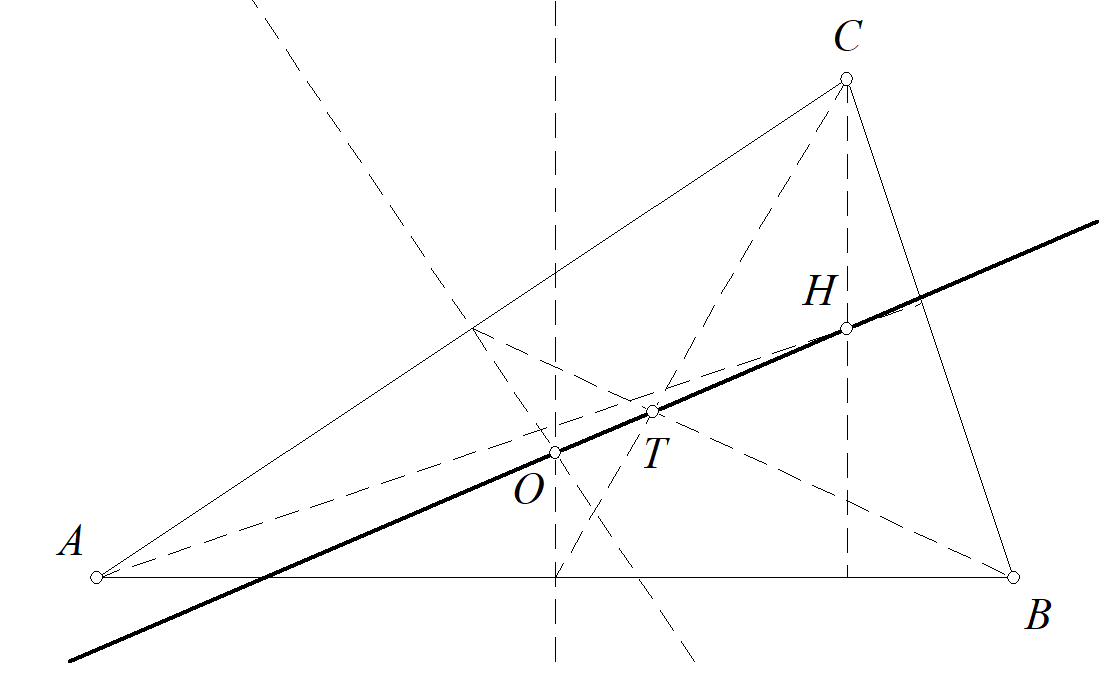
\includegraphics[scale=0.23]{Slike in skice/Eulerjeva_premica.png}
            % \end{figure}

            \begin{figure}
                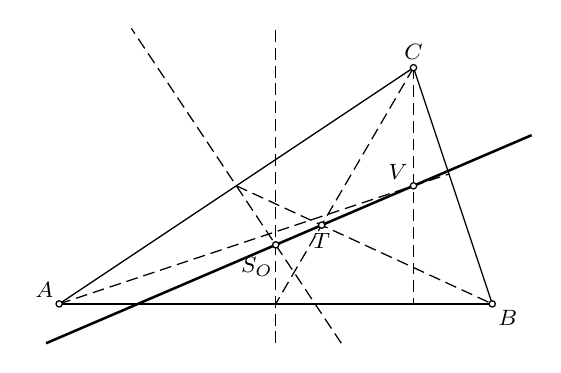
\begin{tikzpicture}
                    % \clip (0,0) rectangle (14.000000,10.000000);
                    {\footnotesize
                    
                    % Drawing segment A B
                    \draw [line width=0.016cm] (1.540000,3.500000) -- (6.960000,3.500000);%
                    
                    % Drawing segment A C
                    \draw [line width=0.016cm] (1.533282,3.522188) -- (5.966718,6.477812);%
                    
                    % Drawing segment B C
                    \draw [line width=0.016cm] (6.987351,3.537947) -- (6.012649,6.462053);%
                    
                    % Drawing line b
                    \draw [line width=0.016cm] (5.083333,3.000000) -- (5.000128,3.124808);%
                    \draw [line width=0.016cm] (4.958526,3.187211) -- (4.875321,3.312019);%
                    \draw [line width=0.016cm] (4.833718,3.374423) -- (4.750513,3.499230);%
                    \draw [line width=0.016cm] (4.708911,3.561634) -- (4.625706,3.686441);%
                    \draw [line width=0.016cm] (4.584103,3.748845) -- (4.500898,3.873653);%
                    \draw [line width=0.016cm] (4.459296,3.936057) -- (4.376091,4.060864);%
                    \draw [line width=0.016cm] (4.334488,4.123268) -- (4.272188,4.216718);%
                    \draw [line width=0.016cm] (4.209681,4.310479) -- (4.126475,4.435287);%
                    \draw [line width=0.016cm] (4.084873,4.497691) -- (4.001668,4.622498);%
                    \draw [line width=0.016cm] (3.960065,4.684902) -- (3.876860,4.809709);%
                    \draw [line width=0.016cm] (3.835258,4.872113) -- (3.752053,4.996921);%
                    \draw [line width=0.016cm] (3.710450,5.059324) -- (3.627245,5.184132);%
                    \draw [line width=0.016cm] (3.585643,5.246536) -- (3.502438,5.371343);%
                    \draw [line width=0.016cm] (3.460835,5.433747) -- (3.377630,5.558555);%
                    \draw [line width=0.016cm] (3.336028,5.620958) -- (3.252823,5.745766);%
                    \draw [line width=0.016cm] (3.211220,5.808170) -- (3.128015,5.932977);%
                    \draw [line width=0.016cm] (3.086413,5.995381) -- (3.003208,6.120189);%
                    \draw [line width=0.016cm] (2.961605,6.182592) -- (2.878400,6.307400);%
                    \draw [line width=0.016cm] (2.836798,6.369804) -- (2.753593,6.494611);%
                    \draw [line width=0.016cm] (2.711990,6.557015) -- (2.628785,6.681823);%
                    \draw [line width=0.016cm] (2.587182,6.744226) -- (2.503977,6.869034);%
                    \draw [line width=0.016cm] (2.462375,6.931438) -- (2.416667,7.000000);%
                    
                    % Drawing line c
                    \draw [line width=0.016cm] (4.250000,3.000000) -- (4.250000,3.150000);%
                    \draw [line width=0.016cm] (4.250000,3.225000) -- (4.250000,3.375000);%
                    \draw [line width=0.016cm] (4.250000,3.450000) -- (4.250000,3.600000);%
                    \draw [line width=0.016cm] (4.250000,3.675000) -- (4.250000,3.825000);%
                    \draw [line width=0.016cm] (4.250000,3.900000) -- (4.250000,4.050000);%
                    \draw [line width=0.016cm] (4.250000,4.125000) -- (4.250000,4.210000);%
                    \draw [line width=0.016cm] (4.250000,4.350000) -- (4.250000,4.500000);%
                    \draw [line width=0.016cm] (4.250000,4.575000) -- (4.250000,4.725000);%
                    \draw [line width=0.016cm] (4.250000,4.800000) -- (4.250000,4.950000);%
                    \draw [line width=0.016cm] (4.250000,5.025000) -- (4.250000,5.175000);%
                    \draw [line width=0.016cm] (4.250000,5.250000) -- (4.250000,5.400000);%
                    \draw [line width=0.016cm] (4.250000,5.475000) -- (4.250000,5.625000);%
                    \draw [line width=0.016cm] (4.250000,5.700000) -- (4.250000,5.850000);%
                    \draw [line width=0.016cm] (4.250000,5.925000) -- (4.250000,6.075000);%
                    \draw [line width=0.016cm] (4.250000,6.150000) -- (4.250000,6.300000);%
                    \draw [line width=0.016cm] (4.250000,6.375000) -- (4.250000,6.525000);%
                    \draw [line width=0.016cm] (4.250000,6.600000) -- (4.250000,6.750000);%
                    \draw [line width=0.016cm] (4.250000,6.825000) -- (4.250000,6.975000);%
                    
                    % Drawing segment C C'
                    \draw [line width=0.016cm] (5.979845,6.465449) -- (5.924419,6.370433);%
                    \draw [line width=0.016cm] (5.886629,6.305650) -- (5.811048,6.176083);%
                    \draw [line width=0.016cm] (5.773258,6.111299) -- (5.697677,5.981733);%
                    \draw [line width=0.016cm] (5.659887,5.916949) -- (5.584306,5.787382);%
                    \draw [line width=0.016cm] (5.546516,5.722599) -- (5.470935,5.593032);%
                    \draw [line width=0.016cm] (5.433145,5.528249) -- (5.357564,5.398682);%
                    \draw [line width=0.016cm] (5.319774,5.333898) -- (5.244193,5.204332);%
                    \draw [line width=0.016cm] (5.206403,5.139548) -- (5.130822,5.009981);%
                    \draw [line width=0.016cm] (5.093032,4.945198) -- (5.017452,4.815631);%
                    \draw [line width=0.016cm] (4.979661,4.750848) -- (4.904081,4.621281);%
                    \draw [line width=0.016cm] (4.866290,4.556497) -- (4.853488,4.534551);%
                    \draw [line width=0.016cm] (4.813178,4.465449) -- (4.790710,4.426931);%
                    \draw [line width=0.016cm] (4.752919,4.362147) -- (4.677339,4.232580);%
                    \draw [line width=0.016cm] (4.639548,4.167797) -- (4.563968,4.038230);%
                    \draw [line width=0.016cm] (4.526177,3.973447) -- (4.450597,3.843880);%
                    \draw [line width=0.016cm] (4.412806,3.779096) -- (4.337226,3.649530);%
                    \draw [line width=0.016cm] (4.299435,3.584746) -- (4.250000,3.500000);%
                    
                    % Drawing segment C U
                    \draw [line width=0.016cm] (6.000000,6.460000) -- (6.000000,6.350000);%
                    \draw [line width=0.016cm] (6.000000,6.275000) -- (6.000000,6.125000);%
                    \draw [line width=0.016cm] (6.000000,6.050000) -- (6.000000,5.900000);%
                    \draw [line width=0.016cm] (6.000000,5.825000) -- (6.000000,5.675000);%
                    \draw [line width=0.016cm] (6.000000,5.600000) -- (6.000000,5.450000);%
                    \draw [line width=0.016cm] (6.000000,5.375000) -- (6.000000,5.225000);%
                    \draw [line width=0.016cm] (6.000000,5.150000) -- (6.000000,5.040000);%
                    \draw [line width=0.016cm] (6.000000,4.925000) -- (6.000000,4.775000);%
                    \draw [line width=0.016cm] (6.000000,4.700000) -- (6.000000,4.550000);%
                    \draw [line width=0.016cm] (6.000000,4.475000) -- (6.000000,4.325000);%
                    \draw [line width=0.016cm] (6.000000,4.250000) -- (6.000000,4.100000);%
                    \draw [line width=0.016cm] (6.000000,4.025000) -- (6.000000,3.875000);%
                    \draw [line width=0.016cm] (6.000000,3.800000) -- (6.000000,3.650000);%
                    \draw [line width=0.016cm] (6.000000,3.575000) -- (6.000000,3.500000);%
                    
                    % Drawing segment A V
                    \draw [line width=0.016cm] (1.537947,3.512649) -- (1.642302,3.547434);%
                    \draw [line width=0.016cm] (1.713454,3.571151) -- (1.855756,3.618585);%
                    \draw [line width=0.016cm] (1.926907,3.642302) -- (2.069210,3.689737);%
                    \draw [line width=0.016cm] (2.140361,3.713454) -- (2.282664,3.760888);%
                    \draw [line width=0.016cm] (2.353815,3.784605) -- (2.496117,3.832039);%
                    \draw [line width=0.016cm] (2.567269,3.855756) -- (2.709571,3.903190);%
                    \draw [line width=0.016cm] (2.780722,3.926907) -- (2.923025,3.974342);%
                    \draw [line width=0.016cm] (2.994176,3.998059) -- (3.136479,4.045493);%
                    \draw [line width=0.016cm] (3.207630,4.069210) -- (3.349932,4.116644);%
                    \draw [line width=0.016cm] (3.421084,4.140361) -- (3.563386,4.187795);%
                    \draw [line width=0.016cm] (3.634537,4.211512) -- (3.776840,4.258947);%
                    \draw [line width=0.016cm] (3.847991,4.282664) -- (3.990294,4.330098);%
                    \draw [line width=0.016cm] (4.061445,4.353815) -- (4.203747,4.401249);%
                    \draw [line width=0.016cm] (4.274899,4.424966) -- (4.417201,4.472400);%
                    \draw [line width=0.016cm] (4.488352,4.496117) -- (4.630655,4.543552);%
                    \draw [line width=0.016cm] (4.701806,4.567269) -- (4.844109,4.614703);%
                    \draw [line width=0.016cm] (4.915260,4.638420) -- (5.057562,4.685854);%
                    \draw [line width=0.016cm] (5.128714,4.709571) -- (5.271016,4.757005);%
                    \draw [line width=0.016cm] (5.342167,4.780722) -- (5.484470,4.828157);%
                    \draw [line width=0.016cm] (5.555621,4.851874) -- (5.697924,4.899308);%
                    \draw [line width=0.016cm] (5.769075,4.923025) -- (5.911377,4.970459);%
                    \draw [line width=0.016cm] (6.037947,5.012649) -- (6.124831,5.041610);%
                    \draw [line width=0.016cm] (6.195982,5.065327) -- (6.338285,5.112762);%
                    \draw [line width=0.016cm] (6.409436,5.136479) -- (6.450000,5.150000);%
                    
                    % Drawing segment B' B
                    \draw [line width=0.016cm] (3.750000,5.000000) -- (3.886194,4.937141);%
                    \draw [line width=0.016cm] (3.954291,4.905712) -- (4.090485,4.842853);%
                    \draw [line width=0.016cm] (4.158582,4.811424) -- (4.294776,4.748565);%
                    \draw [line width=0.016cm] (4.362873,4.717136) -- (4.499066,4.654277);%
                    \draw [line width=0.016cm] (4.567163,4.622848) -- (4.703357,4.559989);%
                    \draw [line width=0.016cm] (4.771454,4.528560) -- (4.797015,4.516762);%
                    \draw [line width=0.016cm] (4.869652,4.483238) -- (4.907648,4.465701);%
                    \draw [line width=0.016cm] (4.975745,4.434271) -- (5.111939,4.371413);%
                    \draw [line width=0.016cm] (5.180036,4.339983) -- (5.316230,4.277125);%
                    \draw [line width=0.016cm] (5.384327,4.245695) -- (5.520521,4.182837);%
                    \draw [line width=0.016cm] (5.588618,4.151407) -- (5.724812,4.088548);%
                    \draw [line width=0.016cm] (5.792909,4.057119) -- (5.929103,3.994260);%
                    \draw [line width=0.016cm] (5.997199,3.962831) -- (6.133393,3.899972);%
                    \draw [line width=0.016cm] (6.201490,3.868543) -- (6.337684,3.805684);%
                    \draw [line width=0.016cm] (6.405781,3.774255) -- (6.541975,3.711396);%
                    \draw [line width=0.016cm] (6.610072,3.679967) -- (6.746266,3.617108);%
                    \draw [line width=0.016cm] (6.814363,3.585679) -- (6.950557,3.522820);%
                    
                    % Marking point A by circle
                    \draw [line width=0.016cm] (1.500000,3.500000) circle (0.040000);%
                    \draw (1.530000,3.470000) node [anchor=south east] { $A$ };%
                    
                    % Marking point B by circle
                    \draw [line width=0.016cm] (7.000000,3.500000) circle (0.040000);%
                    \draw (6.970000,3.530000) node [anchor=north west] { $B$ };%
                    
                    % Marking point C by circle
                    \draw [line width=0.016cm] (6.000000,6.500000) circle (0.040000);%
                    \draw (6.000000,6.500000) node [anchor=south] { $C$ };%
                    
                    % Marking point O by circle
                    \draw [line width=0.016cm] (4.250000,4.250000) circle (0.040000);%
                    \draw (4.320000,4.200000) node [anchor=north east] { $S_O$ };%
                    
                    % Marking point T by circle
                    \draw [line width=0.016cm] (4.833333,4.500000) circle (0.040000);%
                    \draw (4.833333,4.500000) node [anchor=north] { $T$ };%
                    
                    % Marking point H_C by circle
                    \draw [line width=0.016cm] (6.000000,5.000000) circle (0.040000);%
                    \draw (6.030000,4.970000) node [anchor=south east] { $V$ };%
                    
                    % Drawing line O T
                    \draw [line width=0.032cm] (1.333333,3.000000) -- (4.213234,4.234243);%
                    \draw [line width=0.032cm] (4.286766,4.265757) -- (4.796568,4.484243);%
                    \draw [line width=0.032cm] (4.870099,4.515757) -- (5.963234,4.984243);%
                    \draw [line width=0.032cm] (6.036766,5.015757) -- (7.500000,5.642857);%
                    }
                \end{tikzpicture}
                    
            \end{figure}
            

        \end{frame}

        \begin{frame}
            \large\textbf{Vrste trikotnikov -- glede na stranice}
            % ~\\
            \normalsize
            \begin{columns}
                \column<2->{0.35\textwidth}
                \begin{exampleblock}{}
                    RAZNOSTRANIČNI TRIKOTNIK 

                    \begin{figure}
                        \begin{tikzpicture}
                            % \clip (0,0) rectangle (14.000000,10.000000);
                            {\footnotesize
                            
                            % Marking point A by circle
                            \draw [line width=0.016cm] (1.500000,1.500000) circle (0.040000);%
                            \draw (1.500000,1.500000) node [anchor=north] { $A$ };%
                            
                            % Marking point B by circle
                            \draw [line width=0.016cm] (6.000000,1.500000) circle (0.040000);%
                            \draw (6.000000,1.500000) node [anchor=north] { $B$ };%
                            
                            % Marking point C by circle
                            \draw [line width=0.016cm] (4.500000,4.500000) circle (0.040000);%
                            \draw (4.500000,4.500000) node [anchor=south] { $C$ };%
                            
                            % Changing color 255 0 0
                            \definecolor{r255g0b0}{rgb}{1.000000,0.000000,0.000000}%
                            \color{r255g0b0}% 
                            
                            % Drawing segment B C
                            \draw [line width=0.016cm] (5.982111,1.535777) -- (4.517889,4.464223);%
                            
                            % Marking point a
                            \draw (5.250000,3.000000) node [anchor=south west] { $a$ };%
                            
                            % Changing color 0 255 0
                            \definecolor{r0g255b0}{rgb}{0.000000,1.000000,0.000000}%
                            \color{r0g255b0}% 
                            
                            % Drawing segment A C
                            \draw [line width=0.016cm] (1.528284,1.528284) -- (4.471716,4.471716);%
                            
                            % Marking point b
                            \draw (3.000000,3.000000) node [anchor=south east] { $b$ };%
                            
                            % Changing color 0 0 255
                            \definecolor{r0g0b255}{rgb}{0.000000,0.000000,1.000000}%
                            \color{r0g0b255}% 
                            
                            % Drawing segment A B
                            \draw [line width=0.016cm] (1.540000,1.500000) -- (5.960000,1.500000);%
                            
                            % Marking point c
                            \draw (3.750000,1.500000) node [anchor=north] { $c$ };%
                            \color{black}
                            }
                        \end{tikzpicture}
                            
                    \end{figure}

                    vse tri stranice različno dolge 
                    % $\Rightarrow$ vsi trije koti so različni
                    
                \end{exampleblock}
                \column<3->{0.27\textwidth}
                \begin{exampleblock}{}
                    ENAKOKRAKI TRIKOTNIK 

                    \begin{figure}
                        \begin{tikzpicture}
                            % \clip (0,0) rectangle (14.000000,10.000000);
                            {\footnotesize
                            
                            % Marking point A by circle
                            \draw [line width=0.016cm] (1.500000,1.500000) circle (0.040000);%
                            \draw (1.500000,1.500000) node [anchor=north] { $A$ };%
                            
                            % Marking point B by circle
                            \draw [line width=0.016cm] (5.000000,1.500000) circle (0.040000);%
                            \draw (5.000000,1.500000) node [anchor=north] { $B$ };%
                            
                            % Marking point C by circle
                            \draw [line width=0.016cm] (3.250000,5.000000) circle (0.040000);%
                            \draw (3.250000,5.000000) node [anchor=south] { $C$ };%
                            
                            % Changing color 255 0 0
                            \definecolor{r255g0b0}{rgb}{1.000000,0.000000,0.000000}%
                            \color{r255g0b0}% 
                            
                            % Drawing segment B C
                            \draw [line width=0.016cm] (4.982111,1.535777) -- (3.267889,4.964223);%
                            
                            % Marking point a
                            \draw (4.125000,3.250000) node [anchor=south west] { $a$ };%
                            
                            % Drawing segment A C
                            \draw [line width=0.016cm] (1.517889,1.535777) -- (3.232111,4.964223);%
                            
                            % Marking point a
                            \draw (2.375000,3.250000) node [anchor=south east] { $a$ };%
                            
                            % Changing color 0 0 255
                            \definecolor{r0g0b255}{rgb}{0.000000,0.000000,1.000000}%
                            \color{r0g0b255}% 
                            
                            % Drawing segment A B
                            \draw [line width=0.016cm] (1.540000,1.500000) -- (4.960000,1.500000);%
                            
                            % Marking point c
                            \draw (3.250000,1.500000) node [anchor=north] { $c$ };%
                            \color{black}
                            }
                        \end{tikzpicture}
                            
                    \end{figure}

                    dve stranici enako dolgi 
                    % $\Rightarrow$ kota ob osnovnici sta skladna
                    
                \end{exampleblock}                
                \column<4->{0.31\textwidth}
                \begin{exampleblock}{}
                    ENAKOSTRANIČNI ali PRAVILNI TRIKOTNIK 

                    \begin{figure}
                        \begin{tikzpicture}
                            % \clip (0,0) rectangle (14.000000,10.000000);
                            {\footnotesize
                            
                            % Marking point A by circle
                            \draw [line width=0.016cm] (1.500000,1.500000) circle (0.040000);%
                            \draw (1.500000,1.500000) node [anchor=north] { $A$ };%
                            
                            % Marking point B by circle
                            \draw [line width=0.016cm] (5.500000,1.500000) circle (0.040000);%
                            \draw (5.500000,1.500000) node [anchor=north] { $B$ };%
                            
                            % Marking point C by circle
                            \draw [line width=0.016cm] (3.500000,5.000000) circle (0.040000);%
                            \draw (3.500000,5.000000) node [anchor=south] { $C$ };%
                            
                            % Changing color 0 255 0
                            \definecolor{r0g255b0}{rgb}{0.000000,1.000000,0.000000}%
                            \color{r0g255b0}% 
                            
                            % Drawing segment B C
                            \draw [line width=0.016cm] (5.480154,1.534730) -- (3.519846,4.965270);%
                            
                            % Marking point a
                            \draw (4.500000,3.250000) node [anchor=south west] { $a$ };%
                            
                            % Drawing segment A C
                            \draw [line width=0.016cm] (1.519846,1.534730) -- (3.480154,4.965270);%
                            
                            % Marking point a
                            \draw (2.500000,3.250000) node [anchor=south east] { $a$ };%
                            
                            % Drawing segment A B
                            \draw [line width=0.016cm] (1.540000,1.500000) -- (5.460000,1.500000);%
                            
                            % Marking point a
                            \draw (3.500000,1.500000) node [anchor=north] { $a$ };%
                            \color{black}
                            }
                        \end{tikzpicture}
                            
                    \end{figure}

                    vse tri stranice enako dolge 
                    % $\Rightarrow$ vsi trije koti so skladni
                    
                \end{exampleblock}            
            \end{columns}


            \note{
                Enakostranični trikotnik: vse znamenite točke in daljice sovpadajo.
                
                Enakokraki trikotnik: znamenite točke so kolinearne; simetrali osnovnice in kota ob vrhu ter višina in težiščnica osnovnice sovpadajo.
            }
        \end{frame}

        \begin{frame}
            \large\textbf{Vrste trikotnikov -- glede na kote}
            % ~\\
            \normalsize
            \begin{columns}
                \column<2->{0.35\textwidth}
                \begin{exampleblock}{}
                    OSTROKOTNI TRIKOTNIK 

                    \begin{figure}
                        \begin{tikzpicture}
                            % \clip (0,0) rectangle (14.000000,10.000000);
                            {\footnotesize
                            
                            % Marking point A by circle
                            \draw [line width=0.016cm] (1.500000,1.500000) circle (0.040000);%
                            \draw (1.500000,1.500000) node [anchor=north] { $A$ };%
                            
                            % Marking point B by circle
                            \draw [line width=0.016cm] (6.000000,1.500000) circle (0.040000);%
                            \draw (6.000000,1.500000) node [anchor=north] { $B$ };%
                            
                            % Marking point C by circle
                            \draw [line width=0.016cm] (4.500000,4.500000) circle (0.040000);%
                            \draw (4.500000,4.500000) node [anchor=south] { $C$ };%
                            
                            % Drawing segment A B
                            \draw [line width=0.016cm] (1.540000,1.500000) -- (5.960000,1.500000);%
                            
                            % Drawing segment A C
                            \draw [line width=0.016cm] (1.528284,1.528284) -- (4.471716,4.471716);%
                            
                            % Drawing segment B C
                            \draw [line width=0.016cm] (5.982111,1.535777) -- (4.517889,4.464223);%
                            
                            % Changing color 0 0 255
                            \definecolor{r0g0b255}{rgb}{0.000000,0.000000,1.000000}%
                            \color{r0g0b255}% 
                            
                            % Marking point \gamma
                            \draw (4.400000,4.200000) node [anchor=north] { $\gamma$ };%
                            
                            % Marking point \alpha
                            \draw (1.800000,1.500000) node [anchor=south west] { $\alpha$ };%
                            
                            % Marking point \beta
                            \draw (5.800000,1.500000) node [anchor=south east] { $\beta$ };%
                            \color{black}
                            }
                        \end{tikzpicture}
                            
                    \end{figure}

                    ima tri ostre notranje kote
                    
                \end{exampleblock}
                \column<3->{0.29\textwidth}
                \begin{exampleblock}{}
                    TOPOKOTNI TRIKOTNIK 

                    \begin{figure}
                        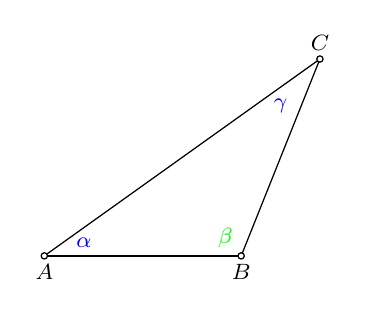
\begin{tikzpicture}
                            % \clip (0,0) rectangle (14.000000,10.000000);
                            {\footnotesize
                            
                            % Marking point A by circle
                            \draw [line width=0.016cm] (1.500000,1.500000) circle (0.040000);%
                            \draw (1.500000,1.500000) node [anchor=north] { $A$ };%
                            
                            % Marking point B by circle
                            \draw [line width=0.016cm] (4.000000,1.500000) circle (0.040000);%
                            \draw (4.000000,1.500000) node [anchor=north] { $B$ };%
                            
                            % Marking point C by circle
                            \draw [line width=0.016cm] (5.000000,4.000000) circle (0.040000);%
                            \draw (5.000000,4.000000) node [anchor=south] { $C$ };%
                            
                            % Drawing segment A B
                            \draw [line width=0.016cm] (1.540000,1.500000) -- (3.960000,1.500000);%
                            
                            % Drawing segment A C
                            \draw [line width=0.016cm] (1.532549,1.523250) -- (4.967451,3.976750);%
                            
                            % Drawing segment B C
                            \draw [line width=0.016cm] (4.014856,1.537139) -- (4.985144,3.962861);%
                            
                            % Changing color 0 0 255
                            \definecolor{r0g0b255}{rgb}{0.000000,0.000000,1.000000}%
                            \color{r0g0b255}% 
                            
                            % Marking point \gamma
                            \draw (4.500000,3.600000) node [anchor=north] { $\gamma$ };%
                            
                            % Marking point \alpha
                            \draw (1.800000,1.500000) node [anchor=south west] { $\alpha$ };%
                            
                            % Changing color 0 255 0
                            \definecolor{r0g255b0}{rgb}{0.000000,1.000000,0.000000}%
                            \color{r0g255b0}% 
                            
                            % Marking point \beta
                            \draw (4.000000,1.500000) node [anchor=south east] { $\beta$ };%
                            \color{black}
                            }
                        \end{tikzpicture}
                            
                    \end{figure}

                    ima en topi notranji kot, ostala dva kota ostra
                    
                \end{exampleblock}                
                \column<4->{0.29\textwidth}
                \begin{exampleblock}{}
                    PRAVOKOTNI TRIKOTNIK 

                    \begin{figure}
                        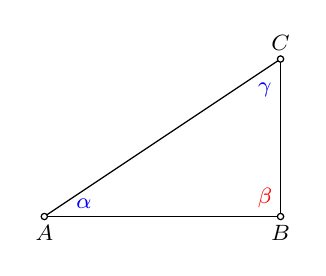
\begin{tikzpicture}
                            % \clip (0,0) rectangle (14.000000,10.000000);
                            {\footnotesize
                            
                            % Marking point A by circle
                            \draw [line width=0.016cm] (1.500000,1.500000) circle (0.040000);%
                            \draw (1.500000,1.500000) node [anchor=north] { $A$ };%
                            
                            % Marking point B by circle
                            \draw [line width=0.016cm] (4.500000,1.500000) circle (0.040000);%
                            \draw (4.500000,1.500000) node [anchor=north] { $B$ };%
                            
                            % Marking point C by circle
                            \draw [line width=0.016cm] (4.500000,3.500000) circle (0.040000);%
                            \draw (4.500000,3.500000) node [anchor=south] { $C$ };%
                            
                            % Drawing segment A B
                            \draw [line width=0.016cm] (1.540000,1.500000) -- (4.460000,1.500000);%
                            
                            % Drawing segment A C
                            \draw [line width=0.016cm] (1.533282,1.522188) -- (4.466718,3.477812);%
                            
                            % Drawing segment B C
                            \draw [line width=0.016cm] (4.500000,1.540000) -- (4.500000,3.460000);%
                            
                            % Changing color 0 0 255
                            \definecolor{r0g0b255}{rgb}{0.000000,0.000000,1.000000}%
                            \color{r0g0b255}% 
                            
                            % Marking point \gamma
                            \draw (4.300000,3.300000) node [anchor=north] { $\gamma$ };%
                            
                            % Marking point \alpha
                            \draw (1.800000,1.500000) node [anchor=south west] { $\alpha$ };%
                            
                            % Changing color 255 0 0
                            \definecolor{r255g0b0}{rgb}{1.000000,0.000000,0.000000}%
                            \color{r255g0b0}% 
                            
                            % Marking point \beta
                            \draw (4.500000,1.500000) node [anchor=south east] { $\beta$ };%
                            \color{black}
                            }
                        \end{tikzpicture}
                            
                    \end{figure}

                    ima en pravi notranji kot, ostala dva kot ostra
                    
                \end{exampleblock}            
            \end{columns}


            \note{
                Pravokotni trikotnik: višinska točka leži v oglišču, ki je vrh pravega kota; središče očrtane krožnice je na razpolovišču hipotenuze; višini katet sta nasprotni kateti; težiščnica na C je enaka polovici hipotenuze.
            }
        \end{frame}


    \subsection{Krog}

        \begin{frame}
            \frametitle{Krog}

            \begin{columns}
                
                \column{0.63\textwidth}
                    \pause
                    \begin{alertblock}{}
                        \textbf{Krožnica} je množica ravninskih točk, ki so enako oddaljene od dane točke $S$. Točko $S$ imenujemo \textbf{središče} krožnice, razdalja $r$ med središčem in poljubno točko na krožnici pa je \textbf{polmer} ali \textbf{radij} krožnice.
                    \end{alertblock}
                    ~\\

                    \pause
                    \begin{alertblock}{}
                        \textbf{Krog} s središčem $S$ in polmerom $r$ je množica ravninskih točk, katerih oddaljenost od središča je manjša ali enaka $r$. To pomeni, da je krog del ravnine omejen s krožnico.
                    \end{alertblock}
        
                \column{0.35\textwidth}
                    \begin{figure}
                        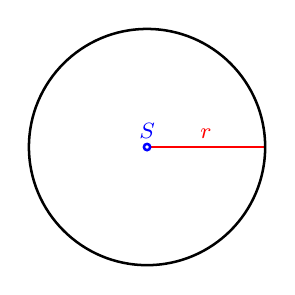
\begin{tikzpicture}
                            % \clip (0,0) rectangle (14.000000,10.000000);
                            {\footnotesize
                            
                            % Changing color 255 0 0
                            \definecolor{r255g0b0}{rgb}{1.000000,0.000000,0.000000}%
                            \color{r255g0b0}% 
                            
                            % Drawing segment S R
                            \draw [line width=0.032cm] (3.040000,3.000000) -- (4.500000,3.000000);%
                            
                            % Marking point r
                            \draw (3.750000,3.000000) node [anchor=south] { $r$ };%
                            
                            % Changing color 0 0 255
                            \definecolor{r0g0b255}{rgb}{0.000000,0.000000,1.000000}%
                            \color{r0g0b255}% 
                            
                            % Marking point S by circle
                            \draw [line width=0.032cm] (3.000000,3.000000) circle (0.040000);%
                            \draw (3.000000,3.000000) node [anchor=south] { $S$ };%
                            
                            % Changing color 0 0 0
                            \definecolor{r0g0b0}{rgb}{0.000000,0.000000,0.000000}%
                            \color{r0g0b0}% 
                            
                            % Drawing circle S R
                            \draw [line width=0.032cm] (3.000000,3.000000) circle (1.500000);%
                            \color{black}
                            }
                            \end{tikzpicture}                            
                    \end{figure}
                    \begin{figure}
                        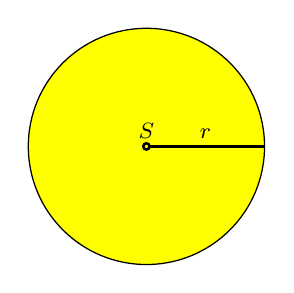
\begin{tikzpicture}
                            % \clip (0,0) rectangle (14.000000,10.000000);
                            {\footnotesize
                            
                            % Changing color 255 255 0
                            \definecolor{r255g255b0}{rgb}{1.000000,1.000000,0.000000}%
                            \color{r255g255b0}% 
                            
                            % Filling circle s
                            \fill (3.000000,3.000000) circle (1.500000);%
                            
                            % Changing color 0 0 0
                            \definecolor{r0g0b0}{rgb}{0.000000,0.000000,0.000000}%
                            \color{r0g0b0}% 
                            
                            % Drawing circle S R
                            \draw [line width=0.016cm] (3.000000,3.000000) circle (1.500000);%
                            
                            % Drawing segment S R
                            \draw [line width=0.032cm] (3.040000,3.000000) -- (4.500000,3.000000);%
                            
                            % Marking point r
                            \draw (3.750000,3.000000) node [anchor=south] { $r$ };%
                            
                            % Marking point S by circle
                            \draw [line width=0.032cm] (3.000000,3.000000) circle (0.040000);%
                            \draw (3.000000,3.000000) node [anchor=south] { $S$ };%
                            \color{black}
                            }
                            \end{tikzpicture}
                            
                    \end{figure}
            \end{columns}
           



        \end{frame}

    \subsection{Štirikotnik}

        \begin{frame}
            \frametitle{Štirikotnik}
        \end{frame}

    \subsection{Večkotnik}

        \begin{frame}
            \frametitle{Večkotnik}
        \end{frame}

    \subsection{Podobnost}

        \begin{frame}
            \frametitle{Podobnost}
        \end{frame}

    \subsection{Podobnost v pravokotnem trikotniku}
        
        \begin{frame}
            \frametitle{Podobnost v pravokotnem trikotniku}
        \end{frame}

    \subsection{Kotne funkcije kotov, velikih od $0^\circ$ do $90^\circ$}
        
        \begin{frame}
            \frametitle{Kotne funkcije kotov, velikih od $0^\circ$ do $90^\circ$}
        \end{frame}
        
    \subsection{Kotne funkcije kotov, velikih od $0^\circ$ do $160^\circ$}
        
        \begin{frame}
            \frametitle{Kotne funkcije kotov, velikih od $0^\circ$ do $360^\circ$}
        \end{frame}
